\documentclass[12pt, a4paper]{report}

\usepackage{dissertation}


%%these packages are not really necessary if you dont need the code and proofs environments
%%so if you like you can delete from here till the next comment
%%note that there are some examples below which obviously won't work once you remove this part
\usepackage{verbatim}
\usepackage{amsfonts}
\usepackage{amsmath}
\usepackage{amssymb}
\usepackage{amsthm}
\usepackage{graphicx}
\usepackage{caption}
\usepackage{subcaption}

\usepackage{afterpage}% http://ctan.org/pkg/afterpage
\usepackage{float}% http://ctan.org/pkg/float
\usepackage{lipsum}% http://ctan.org/pkg/lipsum
\usepackage{color}
\usepackage{fixltx2e}
\usepackage{hyperref}
\usepackage{mathtools}
\usepackage{amsmath}
\usepackage{fancyheadings}
\usepackage{listings}

\definecolor{lightgray}{rgb}{.9,.9,.9}

\lstset{ %
language=MATLAB,                % choose the language of the code
basicstyle=\footnotesize,       % the size of the fonts that are used for the code
numbersep=5pt,                  % how far the line-numbers are from the code
backgroundcolor=\color{lightgray},  % choose the background color. You must add \usepackage{color}
showspaces=false,               % show spaces adding particular underscores
showstringspaces=false,         % underline spaces within strings
showtabs=false,                 % show tabs within strings adding particular underscores
frame=single,           % adds a frame around the code
tabsize=2,          % sets default tabsize to 2 spaces
captionpos=b,           % sets the caption-position to bottom
breaklines=true,        % sets automatic line breaking
breakatwhitespace=false,    % sets if automatic breaks should only happen at whitespace
escapeinside={\%*}{*)}          % if you want to add a comment within your code
}


\pagestyle{fancy}


%%this environment is useful if you have code snippets
\newenvironment{code}
{\footnotesize\verbatim}{\endverbatim\normalfont}

%%the following environments are useful to present proofs in your thesis
\theoremstyle{definition}
\newtheorem{definition}{Definition}[section]
\theoremstyle{definition}%plain}
\newtheorem{example}{Example}[section]
\theoremstyle{definition}%remark}
\newtheorem{proposition}{Proposition}[section]
\theoremstyle{definition}%remark}
\newtheorem{lemma}{Lemma}[section]
\theoremstyle{definition}%remark}
\newtheorem{corollary}{Corollary}[section]
\theoremstyle{definition}%remark}
\newtheorem{theorem}{Theorem}[section]
%%you can delete till here if you dont need the code and proofs environments
\setlength{\headheight}{15pt}


% Begin Document
\begin{document}
%\setcounter{tocdepth}{4}
%\setcounter{secnumdepth}{4}

\newcommand{\hilight}[1]{\colorbox{yellow}{#1}}
% Title Page
\title{Automatic recognition of electrical and architectural symbols using \\ trainable COSFIRE filters}
\author{Luke Agius}
\date{May 2013}
\supervisor{George Azzopardi}
\universitycrestpath{crest_Small}
\submitdate{enter a date} 

% Front sections styling
\frontmatter

% Acknowledgments
\begin{acknowledgements}

I would like to give my thanks to many people who, in one way or an other, have helped me through the completion of this degree and ultimately this dissertation.\\

I would like to first and foremost express my gratitude and appreciation to my supervisor, Dr. George Azzopardi, whose expertise, understanding, and patience, added considerably to my graduate experience. I appreciate his vast knowledge and skill in many areas and his constant assistance and advice in writing this report whilst allowing me the room to work in my own way. \\

Special thanks go to my parents for their constant support, motivation, encouragement through out my studies. Without their help, patience and perseverance I would not be where I am today.\\

I am also thankful for and would like to acknowledge many others who helped me along the way: fellow students for going through this academic journey together, colleagues for sharing ideas and my friends for their patience.\\

\end{acknowledgements}
       

% Table of Contents
\cleardoublepage
\addcontentsline{toc}{chapter}{Table Of Contents}
\tableofcontents

\cleardoublepage
\addcontentsline{toc}{chapter}{\listfigurename}
\listoffigures

\cleardoublepage
\addcontentsline{toc}{chapter}{\listtablename}
\listoftables


% Main Document styling
\mainmatter

% Summary Chapter
\chapter{Summary}

Handheld devices have become ubiquitous due to their flexibility and enhanced productivity. Such devices allow users to write freely on them or to manually sketch symbols. The automatic recognition of handwriting and hand-drawn sketches is important to convert the manual input to a digital representation. Examples of applications include recognition of handwritten letters, digits, signatures, musical notes, electrical and architectural symbols, among others. The objective of this dissertation is to investigate and determine the effectiveness of the COSFIRE filters against isolated symbol recognition with or without degradation applied to the images in question.\\

The approach used, in order to tackle this problem is based upon the work of G.Azzopardi and N.Petkov where a trainable filter, called COSFIRE, inspired by shape-selective neurons in area v4 of the visual cortex. Previously this filter was used successfully in the detection of vascular bifurcations, recognition of handwritten digits and detection and recognition of traffic signs. \\

A thorough literature review is presented which focuses on state-of-the-art symbol recognition methods and covers progress in symbol recognition. Several algorithms are presented along with an explanation on how they work. An introduction about COSFIRE filters is then given to put the reader in context. The COSFIRE filter is then described in detail. This includes the COSFIRE filters' configuration and application stages as well. Also a detailed description is given on how COSFIRE filters are used in the classifier built for this project.\\

Experimental results are then presented which reflect experiments executed against the first three categories of datasets, from the GREC'11 contests, which are publicly available. The following table lists the recognition rates achieved. Results are then interpreted in a discussion which will point out the strengths and weakness of the taken approach. Finally we draw conclusions regarding the effectiveness of COSFIRE filters in isolated symbol recognition. \\

The proposed approach is effective for the automatic recognition of architectural and electrical symbols. It is robust to scalability, noise and geometrical transformations. In most cases it outperforms the state of the art methods for the GREC datasets. In particular, the results that we achieve for the datasets characterised with different levels of degradation and noise are the best ever reported.

% Introduction Chapter
\chapter{Introduction}
\label{chap:intro}

% ===================================== BACKGROUND =====================================================
\section {Background}
\label{sec:background}
Handheld devices have become ubiquitous due to their flexibility and enhanced productivity. Such devices allow users to write freely on them or to manually sketch symbols. Various applications to such devices include the automatic recognition of handwritten letters, digits, signatures, musical notes, electrical and architectural symbols, among others. For instance a musical composer might write down a piece of music on paper or an electrical engineer might also quickly jot down parts of a schematic. Manually converting this handwritten/sketched information into a digital representation may be tedious. \\ 

Such devices enable the composer or the engineer to quickly and efficiently convert their ideas into a correct digital representation. After doing so both the composer and the engineer might be able to quickly incorporate their ideas into a larger, already digitally converted, body of work. For instance, electrical or architectural engineers can quickly convert an image of hand drawn/sketched schematics into a set of symbols and then import them into drafting software such as Auto Cad.\\

Before the recognition process takes place, the document or image in which the manual work is found needs to be segmented. Image segmentation is applied where each symbol is spotted and isolated. This simplifies the recognition process by making the symbol that we need to recognise and classify, more meaningful and easier to analyse.\\

The automatic recognition of isolated symbols, from larger segmented hand-drawn sketches, is an important step in such applications due to the fact that each symbol in physical works need to be properly recognised and converted into a digital representation. This results in a more convenient and efficient storage, retrieval and manipulation as compared to conventional means which consists of starting the sketch from scratch on a computer. \\

A method which has been found to be highly effective for the recognition of isolated patterns is the trainable COSFIRE (Combination Of Shifted FIlter REsponses) approach \cite{Azzopardi_Petkov_2012}. COSFIRE filters, which are effective for keypoint detection and pattern recognition, is trainable as it can be configured by a given contour-based pattern. The configuration process automatically analyses the dominant orientations around the specified prototype. These dominant orientations are detected by the use of Gabor filters. The response of a COSFIRE filter is computed as the weighted geometric mean of the involved Gabor filter responses. This means that a response is only achieved when all the concerned contour parts are present.The COSFIRE approach can also achieve invariance to rotation, scale, reflection and contrast inversion. \\

In their paper \cite{Azzopardi_Petkov_2012}, the authors demonstrated that a shape descriptor can be formed with the collective responses of multiple COSFIRE filters. They have also demonstrated that COSFIRE filters can be effectively applied to the detection of vascular bifurcations, recognition of handwritten digits and detection and recognition of traffic signs in complex scenes. In this work, we investigate the effectiveness of the mentioned COSFIRE filters for the recognition of electrical and architectural symbols.
    
% ===================================== RESEARCH QUESTIONS =====================================================    
\section {Research Questions} 
The following are the questions that we investigate in this work:-
    \begin{enumerate}
        \item How effective are COSFIRE filters for the recognition of electrical and architectural symbols?
        \item How robust are COSFIRE filters to noisy symbols?
        \item How does the results achieved by COSFIRE filters compare to published result of state-of-the-art methods?
    \end{enumerate}

The effectiveness of COSFIRE filters is evaluated by numerous experiments which are performed on various publicly available data sets \cite{Delalandre_contest} \cite{Delalandre_sketched}. These data sets hold 150 different classes of symbols. Every data set contains a model symbol for each class and many test images that we use for evaluation. Test symbols, are then used to test the configured COSFIRE filters. The test symbols contain both noisy and noise less symbols. Furthermore, some test symbols are scaled or/and rotated.

% ===================================== DELIVERABLES =====================================================    
\section {Deliverables}
In this thesis, the deliverables include a description of the proposed method and a comparison against other state of the art techniques. The three posed research questions will be addressed by various experiments implemented on Matlab followed by in depth analysis of the results. Performance measurements will be computed in the form of true positives and false positive rates which can be used to derive accuracy, precision and recall rates. Documentation of the MATLAB implementation is provided on how it is built, Section \ref{sec:built}. This also includes a step by step guide on how to re-run the experiments, Section \ref{sec:howto}. The needed files are included in the CD, Section \ref{sec:CD}. A discussion is included concerning some aspects of the proposed approach which highlights the differences that distinguish it from other approaches. Finally, we draw conclusions and provide an outlook of future work.

% ===================================== PROJECT PLAN =====================================================    
\section {Project Plan}

\begin{figure}[H]
    \centering
    \includegraphics[angle=90,totalheight=0.89\textheight, keepaspectratio]{figures/introduction/capture.png}
    \caption[Thesis Project Plan]{Project Plan}
    \label{fig:projectplan}
  \end{figure}
  
Fig. \ref{fig:projectplan} shows the project plan for this thesis. The actual project plan deviated a little from the original one in terms of duration for certain tasks. Tasks other than the experiments required less time such as searching for adequate datasets, the building of the classifier and writing the preliminary report. The deviation in terms of task duration took place due to the fact that the some experiments required more time than actually planned because of the size of the data set to be processed and the number of computations done for each data set. \\

Therefore, due to time restrictions and having datasets with a larger number of classes available, which require more time to process,  not all datasets where classified  within the allotted time frame. This is explained further in Chapter \ref{chap:disc} Discussion.

\section {Overview of The Report}
Below is a brief outline for each chapter of this dissertation. \\
  
{\bf Chapter 2 - Literature Review} \\
The literature review focuses on state-of-the-art symbol recognition methods and presents an overview of several published algorithms used and results obtained. The research covers the progress in this area of research and discusses potential future work.\\

{\bf Chapter 3 - Methodology} \\
This chapter is divided into two main sections. The first section gives a detailed description of COSFIRE filters. It explains the COSFIRE filters' configuration and application stages in detail.\\

The second section is the Evaluation section, which gives a detailed description of how COSFIRE filters are used in the classification of electrical and architectural symbols. This section is further divided into five sections were, the data sets, pre-processing, configuration of COSFIRE filters, forming a shape descriptor and the classification technique used are explained in detail.\\

{\bf Chapter 4 - Experimental Results} \\
This section provides the results obtained for various data sets of different complexity. \\


{\bf Chapter 5 - Discussion} \\
This section provides a discussion about the proposed method to the recognition of isolated symbols in hand drawn images. We also compare our results with those obtained by other state of the art methods. \\

{\bf Chapter 6 - Summary Conclusion} \\
This chapter provides a summary of the entire dissertation. Subsequently conclusions are drawn.
  
    
% Literature Review Chapter    
\chapter{Literature Review}
\label{chap:literature}

\section {Overview}
\label{sec:overview}

With the widespread popularity of portable digital input devices like smartphones and tablets, there is increasing interest in the development of systems that can automatically interpret and convert paper based graphical information into an equivalent digital representation. This conversion to digital representations has been a topic of active research throughout the last decade \cite{Cordella_2000} \cite{Delalandre_2012}. \\

A fundamental way in which we communicate information, especially technical information, is through the use of diagrams \cite{Ouyang_2009}. Much of this effort is focused on the automatic conversion of manually sketched work / diagrams to a digital format which can be understood by CAD systems in order to be included into other larger bodies of work. \\

A key issue, at the heart of such research efforts, is the recognition of domain dependant symbols using domain-independent techniques. Authors commonly develop ad-hoc techniques which are difficult to reuse in other domains \cite{Llados}. Various approaches have been proposed to solve this issue, however challenges remain in terms of finding a general and efficient method which can be applied across domains with well establish performance and recognition accuracy. \\ 


In this literature review we direct our focus on the recognition of symbols from the electrical engineering and architectural domains. The main goal is to explain the process of symbol recognition in detail and then to highlight the different approaches adopted to-date to solve the problem of symbol recognition. \\


\section{What Is a Symbol?}
\label{sec:whatis}
The oxford dictionary defines the word 'symbol' as a mark or character which is used as a conventional representation of an object, function or process. In a very general way, a symbol can be defined as a contextually meaningful graphical shape of a specific application domain \cite{Llados}. Depending on the application, we can find various kinds of symbols in different industry fields like architecture, cartography, 
electronics, engineering etc. Each field use domain-dependant notations to construct their symbol designs. \\

In technical fields such as in architecture and engineering, symbols are designed in 2-dimensions (2D) using domain dependant notation \cite{Llados}.Simple symbols can be binary, made out of sets of line segments, both straight and in loops, such as electrical or architectural symbols , Fig. \ref{fig:electrical}. Symbols can also be complex, involving different levels of colours and shades, such as company logos \cite{Cordella_2000}, Fig. \ref{fig:logo}. \\

\begin{figure*}[h]
        \centering
        \begin{subfigure}[b]{0.4\textwidth}
                \centering
                \includegraphics[width=0.5\textwidth]{figures/introduction/electricalsymbol.jpg}
                \caption{}
                \label{fig:electrical}
        \end{subfigure}
        \begin{subfigure}[b]{0.4\textwidth}
                \centering
                \includegraphics[width=0.5\textwidth]{figures/introduction/logosymbol.jpg}
                \caption{}
                \label{fig:logo}
        \end{subfigure}
        \caption[Example of Symbols]{(a) An example of a contour based symbol and (b) An example of a complex symbol}
        \label{fig:symbolexamples}
\end{figure*}

From a symbol recognition stand point, documents of interest which mostly hold the most symbols can be grouped into three main categories \cite{Cordella_2000} :-

    \begin{enumerate}
        \item Technical drawings, such as flow diagrams and electrical schematics, Fig \ref{fig:electrical}
        \item Maps, topographical or geographical, Fig \ref{fig:map}
        \item Others, such as musical glyphs, Fig \ref{fig:score}
    \end{enumerate}

Symbols in such documents are formed depending on various domain dependent rules\cite{Cordella_2000}. Furthermore, when presented, they can contain added noise, be deformed, incomplete, and/or geometrically transformed. Symbols may also appear in isolation or in complex backgrounds. They may be in close proximity, touching or partially overlap each other. \\

\begin{figure*}[h]
\centering
    \begin{subfigure}[b]{0.4\textwidth}
        \centering
        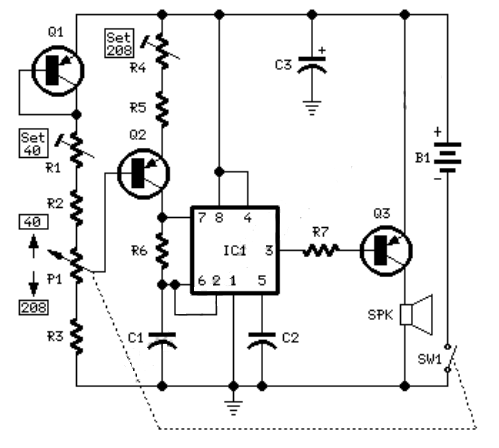
\includegraphics[width=1\textwidth]{figures/LitreatureReview/schematic.png}
        \caption{}
        \label{fig:electrical}
    \end{subfigure}
    \begin{subfigure}[b]{0.4\textwidth}
        \centering
        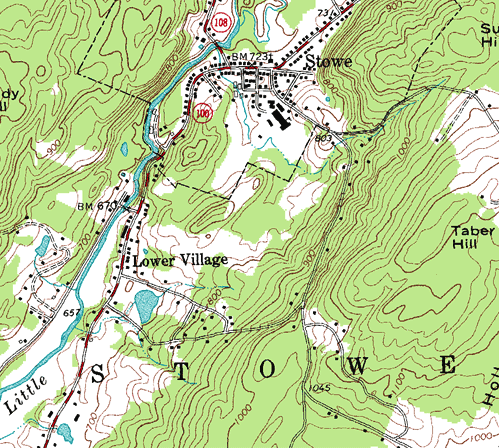
\includegraphics[width=1\textwidth]{figures/LitreatureReview/map2.png}
        \caption{}
        \label{fig:map}
    \end{subfigure}
        \begin{subfigure}[b]{0.4\textwidth}
        \centering
        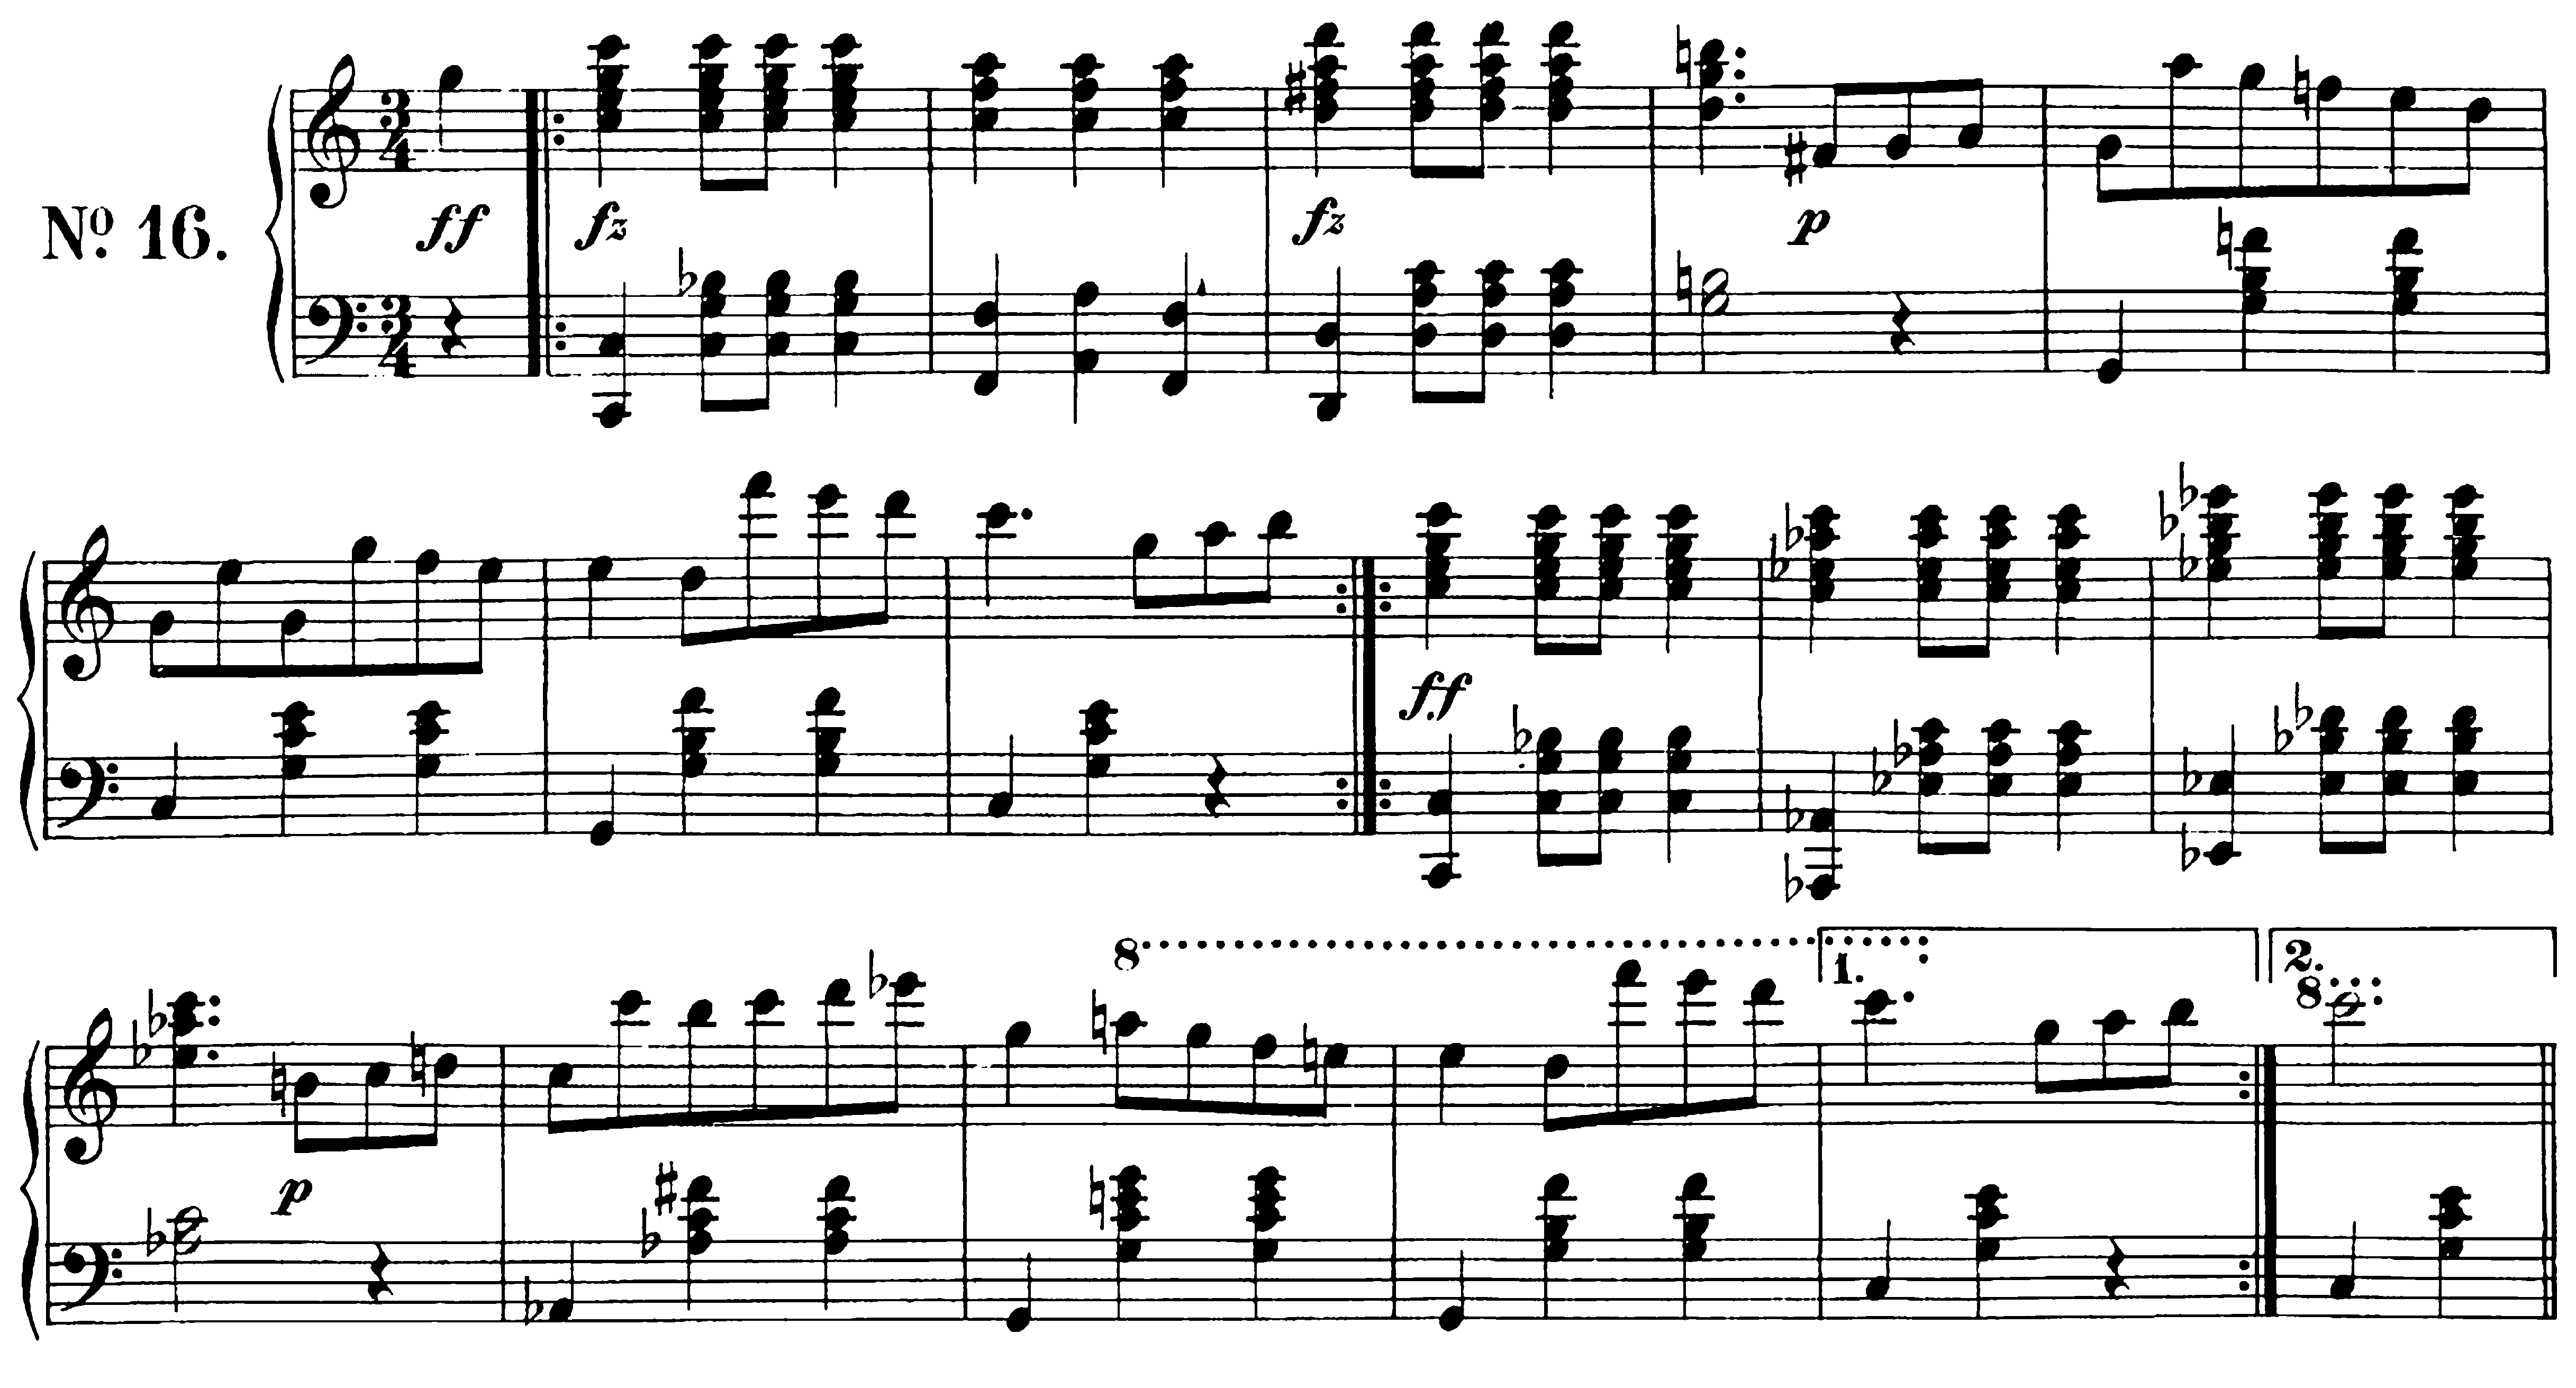
\includegraphics[width=1\textwidth]{figures/LitreatureReview/score2.png}
        \caption{}
        \label{fig:score}
    \end{subfigure}
    
    \caption[Example of symbol holding documents]{Different types of documents in which symbols are found such as (a) Electric schematics\footnotemark, (b) topographical map\footnotemark, (c) musical scores\footnotemark.}
    \label{fig:documentexamples}
\end{figure*}

\vspace{19mm}
\footnotetext[1]{Taken From \url{http://www.redcircuits.com/Page8.htm}}
\footnotetext[2]{Taken From \url{http://en.wikipedia.org/wiki/File:Topographic_map_example.png}}
\footnotetext[3]{Taken From \url{http://music.unt.edu/mhte/theory/TF}}


\section{Symbol Recognition}
Information is shared in many forms. It is often represented by textual or graphical means. At the core of human learning, lies the ability of pattern recognition and inference. This ability helps us to process information in any form it is presented, be it textual, graphical or otherwise. \\

In Artificial Intelligence (AI) research a constant effort is being put forward in order to model and automate these abilities by mechanical means \cite{duin2007science}. 
The successful modelling of such abilities yield various advantages. As described in Section \ref{sec:background}, such advantages include the automatic conversion of paper-based information into a equivalently meaningful digital version. This results in more convenient, efficient retrieval and manipulation of the information in question. In various fields, such as architecture, electronics, cartography, etc, information is conveyed in a diagrammatic form \cite{Llados}. Symbols constitute an important informative source in diagrams \cite{XML} and depending on the field and the application being used, different symbols can be found.  These symbols can be designed according to domain dependent rules or none at all. \\

This problem is tackled through symbol recognition. Symbol recognition is a field within pattern recognition area to which a lot of research effort has been devoted \cite{musings}. It is the automatic process where an input image of unknown pattern is classified to a particular class in a particular domain. \cite{Llados} \cite{luqman_2009}. This process is then used in the conversion of paper based graphical symbols into equivalent digital representations.\\

The process of symbol recognition can be divided into two main parts namely segmentation and recognition. The first part, segmentation of the document or image, is a prerequisite to the second part, recognition. Segmentation isolates the symbols from the document or image, for an easier and computationally lighter recognition process.\\

Combining segmentation and recognition into one system is one of the main problems within the field of symbol recognition. This problem is known as the "segmentation/recognition paradigm" \cite{delal2}. This problem describes that a document or image should be segmented before recognition can take place. However, at the same time, some kind of recognition needs to be applied for segmentation to take place \cite{yoon2001new}. \\

An other pre-requisite is that a system needs some priori knowledge about the symbols it needs to recognise in order to successfully recognise symbols \cite{delal2}. This corresponds to learning a database of model symbols for training purposes. Various shape recognition methods have been applied for this training phase. \\

Symbol recognition can be classified into two main categories, statistical and structural. Structural symbol recognition is based on the organisation of primitives, such as straight lines and arcs, into higher defined structures such as symbols or signatures \cite{ogierRobustSymbolRecognition}. On the other hand statistical symbol recognition is based on representing the symbol in simpler forms by the use of a shape descriptor \cite{Llados}. The following sub sections explain those two categories in detail.


\subsection{Statistical Symbol Recognition}
In a statistical approach towards symbol recognition, each symbol is represented by a unique signature. This signature is in the form of a feature vector of $n$ dimensions extracted from the same symbol. This approach has two important issues. The first issue is the selection of features for every pattern and the second one is the partitioning of the feature space \cite{Llados}. In this case, the feature space refers to the set of model symbols available.\\

The feature vector for every symbol is constructed depending on the properties of the inputted pattern. The chosen set of features for each symbol must be unique. This is critical to attain high discrimination power thus ultimately avoiding confusion between symbols in the classification process \cite{Llados}.\\

There are various methods with which a set of features is extracted from a pattern or symbols such as: centroids, line intersections, projection profiles, etc, amongst many \cite{Llados}. These methods adopt an invariant approach towards added noise, geometrical image transformations and distortions \cite{Llados}.Once that a set of features is chosen for each symbol, classification consists in choosing a segmentation method in order to partition the feature space. This is done on order to assign each feature vector to one of the available classes. \\

One of the simplest feature spaces is the image space it self, where the feature vector is composed of features each corresponding to a pixel with in the image. When an image is used as a feature space it is usually normalised to a certain size \cite{Llados}. Although this is one of the simplest feature spaces to process it has a number of advantages. It is simpler to process due to its low complexity, moreover it corresponds directly to the input information's visual appearance. However, it also has a number of disadvantages. This feature space does not adhere to an intravariant approach, therefore it does not take into consideration image distortion or geometrical transformations. Furthermore, it is very sensitive to noise. \\

The simplest way to partition a feature space consists in defining a distance function among the available feature vectors. This can be done by using the k-nearest neighbour algorithm (KNN). Which distance function to use in the Knn algorithm, depends on the application. One of the most popularly used distance functions is the Euclidean distance. The KNN algorithm is based on the concept of similarity \cite{Llados}. It takes into account the nearest $K$ number of neighbours which can weight in, in the classification of the presented pattern. Other methods have also been used for the classification of unknown patterns which are also based on the concept of similarity such as neural networks \cite{ANNS} and decision trees \cite{decisiontrees}.\\

Artificial neural networks (ANNs) have been proven to be adequate for classification purposes often achieving good recognition rates across various domains. One of the advantages in ANNs is their learning capabilities. They adapt quickly to the properties of the provided training set \cite{Llados}. \\

Decision trees for the purpose of symbol recognition are constructed in such a way that each of node in the tree corresponds to a particular feature. Classification is then carried out by visiting the nodes which satisfy a condition with the inputted image. This approach follows the tree branches which ultimately lead to a leave node which corresponds to a recognised symbol \cite{Llados}. \\

The main goal is to minimise, as much as possible, the distance between the input pattern and the pattern class it belongs to. At the same time, the distance between the same input pattern and other pattern classes is maximised \cite{Llados}.

\subsection{Structural Symbol Recognition}
In the structural approach towards symbol recognition, symbols are represented by a description of their shape in terms of simpler parts and the relationship between them \cite{Llados}. These parts are geometric primitives \cite{zernike} which usually consist of straight lines and arcs. However other geometric primitives have been also used such as loops, contours or simple shapes such as circles, rectangles etc. \\

Since the symbol is described by the geometric primitives it contains, a previous vectorization step is required. Vectorization is the process by which a raster image is converted into a set of geometrical primitives described above. Vectorization of raster images introduces both noise and distortion in the symbol's representation\cite{Llados}. \\

As cited in \cite{Llados} there is a large body of work about structural approaches focusing on symbol graph representation \cite{Groen, hamada, mediangraph,combi,graphmatch,engdrawings,1997combining}. When representing a symbol with a graph, each node and edge correspond to points and lines within the image. This provides a natural and intuitive symbol description. Classification for these methods consist in finding the best matching subgraphs between the input symbol and the models of the symbols. One of the main drawbacks for this method is its computational complexity. However some ways of reducing computation have been explored \cite{Llados}.\\

An other method of symbol representation in various structural approaches is by defining formal grammars. Graph grammars are the most common because of bi-dimensional structure of symbols \cite{Llados}. A grammar stores in a very compact manner all valid instances of a symbol or a class of symbols. Correct classification then consists of parsing its representation in order to test whether it can be generated by defined grammar. Grammars are useful in applications where the shape of the symbols can be accurately defined by a set of rules, for example technical drawings.\\

An other method which has also been used in structural approaches is the use of Hidden Markov Models (HMMs). HMMs is a powerful statistical tool for modelling generative sequences \cite{markovs}. HMMs are used since the structure of the symbol can be described as a sequence of states which generate the image. Recognition then consists in finding the sequence of states with the higher probability.

\subsection{Performance Evaluation}
\label{sec:perf}
During the last decade, attention has been shifted in the development of a generic and standard framework which permits the comparison and performance evaluation of symbol recognition methods. This effort has resulted in various contests such as the GREC contests taking place  which focus on the recognition of isolated symbols and thus creating a framework for evaluation reasons \cite{Delalandre_2012}.

\subsubsection{Datasets}
    
For the evaluation and comparison of the methods used in these contests, publicly available data sets of isolated symbols are generated \cite{Delalandre_contest} \cite{Delalandre_sketched}. These datasets are generated with a set of goals in mind \cite{Delalandre_contest}:

   \begin{enumerate}
        \item To provide a set of tests that could evaluate scalability of methods.
        \item To be able to test the performance of methods under some realistic increasing depredations.
        \item  To be able to test the generalisation ability of the methods.
    \end{enumerate}

The generated data sets are organised into four categories which have different levels of complexity due to noise, deformation, rotation and scaling. The first category consists of 24 data sets. Each data set contains a number (varying between 25 and 150) of different electrical and architectural symbols each represented by a single image. These data sets contain 1000 test images of deformed symbols of increasing complexity. For instance, the least complex data set contains images that are only slightly deformed, while the most complex data set consists of images of symbols with the highest deformation.\\

The second category consists of 3 datasets each having 150 different symbols. These datasets contain test symbols with geometrical transformation applied such as scaling, rotation or combined. The third category of datasets consists of 3 datasets each comprising of 150 different models as well with three different kinds of noise applied separately. \\

The method used to apply noise to the test images was proposed by Kanungo \cite{888707}. The remaining data sets contain images of geometrically transformed symbols, such as different orientations and scale. Fig. \ref{fig:noises} shows a sample of the test images with noise applied.

\begin{figure*}[h]
        \centering
        \fbox{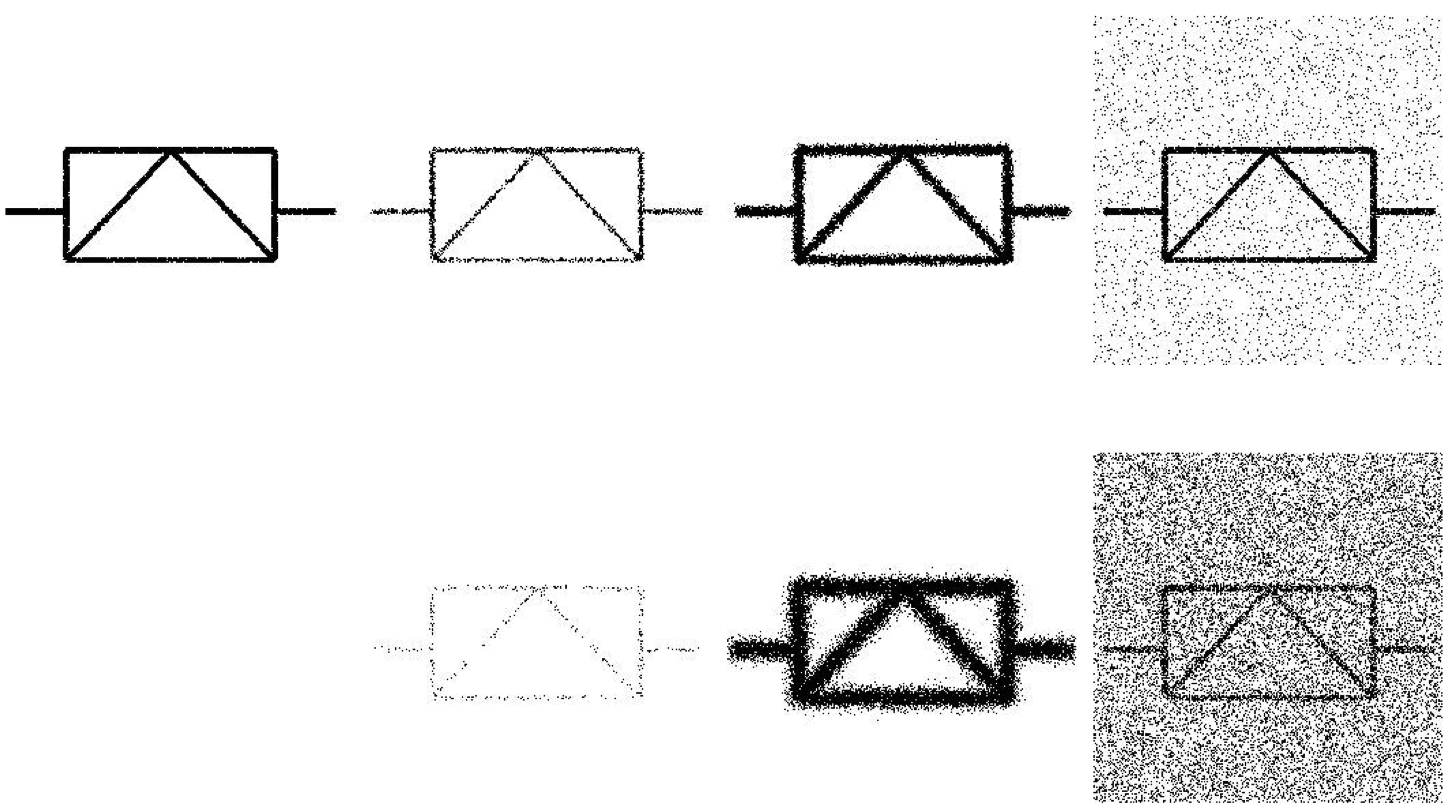
\includegraphics[width=0.5\textwidth]{figures/LitreatureReview/noises.png}}
        \caption[Sample test images which include noise]{A sample set of test images for the model, found at the top left corner of the image, with noise applied according to Kanungo's method \cite{888707}. Adapted from \cite{Delalandre_contest}.}
        \label{fig:noises}
\end{figure*}

The last, fourth, category contains three data sets. They contain large number of different model symbols and large number of test images that combine different degradation levels and different transformations \cite{Delalandre_2012}.

\subsubsection{Performance Metrics}
For the symbol recognition contest the chosen performance metric was the recognition rate \cite{Delalandre_2012}. The recognition rate is determined by counting the true positives (TP) and the false positives (FP). The recognition rate is then calculated as follows, where $R$ is the recognition rate in percentage.

\begin{equation}
    R = \left(\frac{1}{(TP+FP)} \times TP\right) \times 100
\end{equation}

\subsubsection{Results}
The authors report that only one participant submitted a method which approached both symbol spotting and recognition \cite{Nayef}. Amongst the global results reported, the following results are the ones attained by testing the second and third category of datasets. For each kind of deformation and noise a different result was attained. \\

\begin{table}[h]
\centering
\caption{Contest's results for the second category of datasets.}
\begin{tabular}{ccccccccccccccc}
  \hline
      Degradation & & & & & & & & Recognition Rate \\
  \hline
      Rotation & & & & & & & &  81.07 \% \\
      Scaling & & & & & & & &  89.20 \% \\
      RotationScaling & & & & & & & &  84.27 \% \\   
  \hline
\end{tabular}
\end{table}


\begin{table}[h]
\centering
\caption{Contest's results for the third category of datasets.}
\begin{tabular}{ccccccccccccccc}
  \hline
      Degradation & & & & & & & & Recognition Rate \\
  \hline
      Noise A & & & & & & & &  88.07 \% \\
      Noise B & & & & & & & &  85.73 \% \\
      Noise E & & & & & & & &  85.67 \% \\   
  \hline
\end{tabular}
\end{table}
      

The authors think that the datasets used in their work, can serve future similar contests as a stable platform against which evaluation and comparison  of symbol recognition methods can be done. Future editions will hold hand drawn symbols \cite{Delalandre_2012}.


\section {State of The Art}

Shape descriptors have been used in a variety of applications and tasks such as shape analysis, comparison and retrieval \cite{Heider}. In symbol recognition, as previously described, shape descriptors are an integral part of the process. The goal of the shape descriptor is to represent a pattern by a unique structure which relies on the extraction of local or global features. \\

As observed in previous studies \cite{Alajlan}, shape descriptors can be either global or local. Global shape descriptors take into consideration the entire shape of the object while local shape descriptors are used for local shape features \cite{wang}.Shape descriptors which are either global or local may fail to be robust. Global descriptors are reported to be robust to local deformations, but fail when trying to capture local shape details. At the same time local descriptors are adequate in representing local shape features, however they are very sensitive to noise \cite{wang}. \\

One of the most important challenges in shape descriptors is to come up with a solution by defining a rich shape descriptor, which consists of both Global and local properties. This solution needs to be computationally fast and efficient, compact, and most importantly, general enough to be used in a variety of applications.

The features that a shape descriptor detects represent information about specific structures within the image or pattern itself. This information ranges from simple geometric primitives such as point or edges to much more complex ones such as objects or a set of primitives. The extraction of such features is a very critical problem in computer vision and is used widely in various vision related tasks such as object recognition and tracking \cite{Maji_comparison}. Due to their importance, a lot of research attention has been dedicated to it \cite{Heider, Maji_comparison}. \\

Depending on the application an intravariant approach towards feature extraction becomes important. One of the most important jobs of a shape descriptor is to extract unique features which are both repeatable as well as invariant to various conditions such as noise or distortion. Apart from this a good shape descriptor should be informative, discriminative and efficient in matching process \cite{wang}. The rest of this section reviews a number of feature descriptors applied to date. \\

A very popular shape descriptor is the Shape Context approach. It is feature descriptor which was proposed by S. Belongie and J. Malik in 2000 \cite{context}. Given a collection of points within an image which have been extracted from a set of detected edge elements, the shape context descriptor captures the relative distribution of points in the plane relative to each point on the shape \cite{contextWeb}. \\

A very popular shape descriptor is the Shape Context approach. It is feature descriptor which was proposed by S. Belongie and J. Malik in 2000 \cite{context}. Given a collection of points within an image which have been extracted from a set of detected edge elements, the shape context descriptor "captures the relative distribution of points in the plane relative to each point on the shape" \cite{contextWeb}. \\

The shape context approach operates on the concept of similarity where it is measured between shapes and exploited for pattern recognition purposes. For example, when taking into account two written digits, Fig \ref{fig:similarity}, interpretation can differ. When taken as a set of pixel with various brightness values, the two digits are very different. However when observed by a human, they appear to be very similar.


\begin{figure*}[h]
        \centering
        \fbox{
\includegraphics[width=0.2\textwidth]{figures/LitreatureReview/similiar.png}}
        \caption[An example of similarity]{Two written digits can be interpreted differently depending who the observer is. Adapted from \cite{context}.}
        \label{fig:similarity}
\end{figure*}

The aim of the authors is to put into operation the concept of similarity for object classification. This approach is described as a three stage process \cite{context}:

\begin{enumerate}
    \item "Solve the correspondence problem between the two shapes"
    \item "Use the correspondences to estimate an aligning transform"
    \item "Compute the distance between the two shapes as a sum of matching errors between corresponding points, together with a term measuring the magnitude of the aligning transformation"
\end{enumerate}

At the core of the similarity concept that the authors use in their work is the fact that it has been observed that shapes which are related but not identical, can often be deformed to a point where they are aligned using simple coordinate transformations, Fig. \ref{fig:fish}. Therefore, based on this the authors have come up with an algorithm which finds correspondences between similar shapes. \\

\begin{figure*}[h]
        \centering
        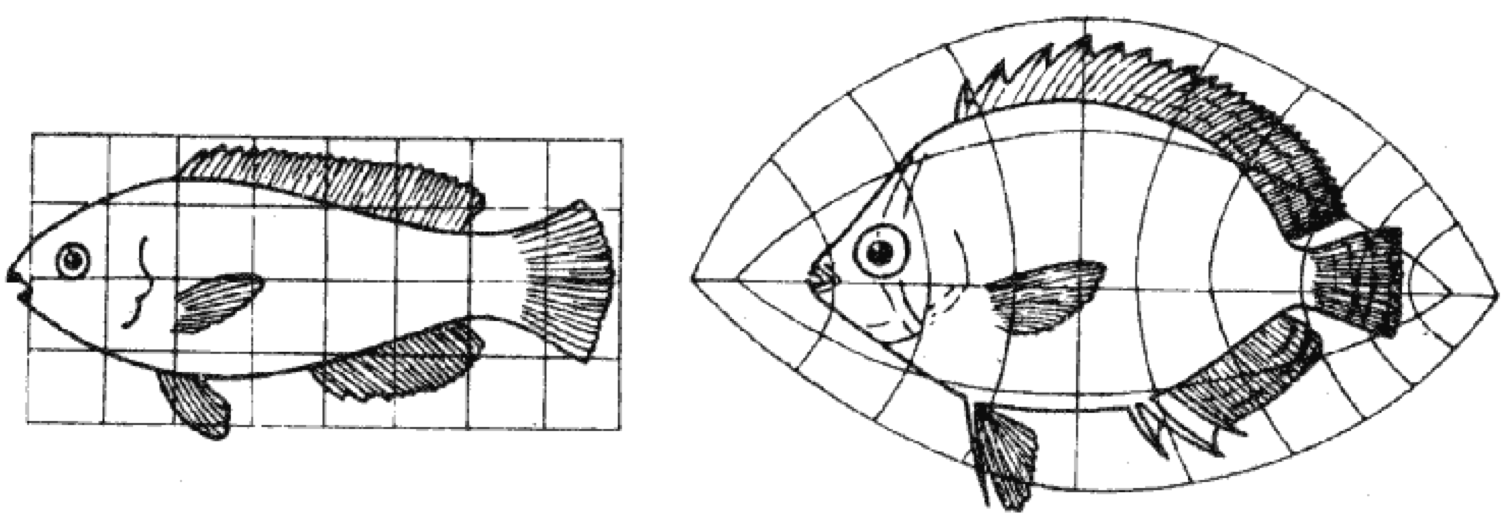
\includegraphics[width=0.9\textwidth]{figures/LitreatureReview/fish.png}
        \caption[An example of simple coordinate transformations between similar objects]{An example of coordinate transformation between two similar objects. Adapted from \cite{context}.}
        \label{fig:fish}
\end{figure*}

In this approach, shapes are represented by a collection of points. This collection of $n$ number of points is sampled from the shape's contours by using an edge detector. When these points are taken into consideration on their own, they hold no particular importance.\\

\begin{figure*}[h]
        \centering
        \begin{subfigure}[b]{0.36\textwidth}
                \centering
                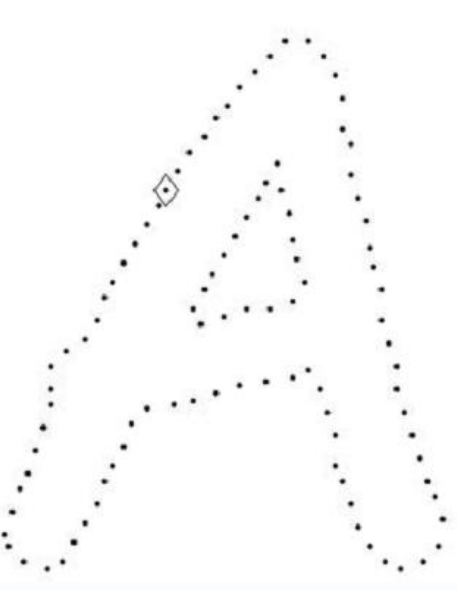
\includegraphics[width=0.6\textwidth]{figures/LitreatureReview/letter.png}
                \caption{}
        \end{subfigure}
        \begin{subfigure}[b]{0.36\textwidth}
                \centering
                \includegraphics[width=0.7\textwidth]{figures/LitreatureReview/letterpoints.png}
                \caption{}
        \end{subfigure}
        \caption[Point selection and calculated distribution shape context descriptor]{(a) A point is selected from a collection of points representing the shape. (b) Using a diagram of log-polar histogram bins we compute the point distribution and thus the shape contexts. Adapted from \cite{context}.}
        \label{fig:contextPart1}
\end{figure*} 

The shape context descriptor then describes the distribution of the rest of the shape relative to a selected point by placing a diagram of log-polar histogram bins on the selected point, Fig. \ref{fig:contextPart1}. The histogram is divided into a number of bins. From each of these bins the number of points is counted. This will describe the spatial arrangement of point around the selected point. When the selected shape needs to be matched to an other shape, the same procedure is applied to the other shape. Once this is done the arrangement attained from one shape is compared to the other one. Fig. \ref{fig:contextPart2} shows two different shapes of similar shape. From each a point has been chosen to check for correspondence between the two shapes.\\ 

\begin{figure*}[h]
        \centering
        \begin{subfigure}[b]{0.36\textwidth}
                \centering
                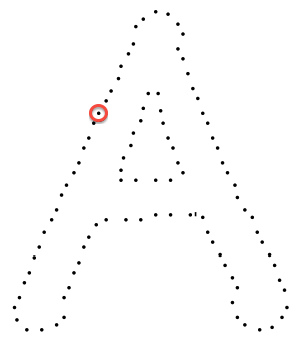
\includegraphics[width=0.7\textwidth]{figures/LitreatureReview/lettera.png}
                \caption{}
                \label{fig:lettA}
        \end{subfigure}
        \begin{subfigure}[b]{0.36\textwidth}
                \centering
                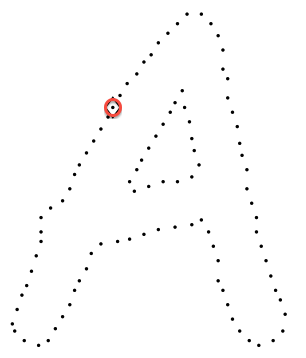
\includegraphics[width=0.7\textwidth]{figures/LitreatureReview/letterb.png}
                \caption{}
                \label{fig:lettB}
        \end{subfigure}
        \caption[Choice of points from two similar shapes for calculation of shape context]{(a) A Point is selected from a shape to be compared to (b) an other point from a similar shape. Adapted from \cite{context}.}
        \label{fig:contextPart2}
\end{figure*}

For each point a shape context is calculated as a log-polar histogram of the coordinates of the rest of the collection of points using the selected point as the origin, Fig. \ref{fig:contextPart3}.\\

\begin{figure*}[h]
        \centering
        \begin{subfigure}[b]{0.36\textwidth}
                \centering
                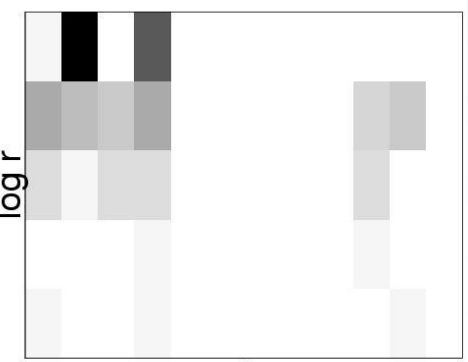
\includegraphics[width=0.7\textwidth]{figures/LitreatureReview/responsea.png}
                \caption{}
        \end{subfigure}
        \begin{subfigure}[b]{0.36\textwidth}
                \centering
                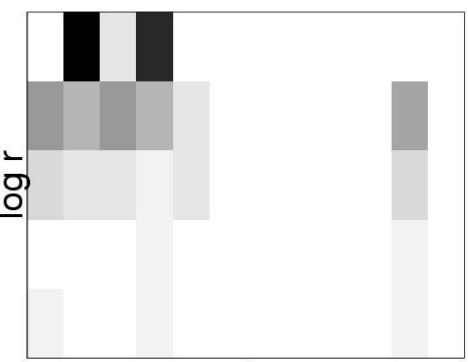
\includegraphics[width=0.7\textwidth]{figures/LitreatureReview/responseb.png}
                \caption{}
        \end{subfigure}
        \caption[Shape context result for two points from two similar shapes]{(a) Shows the shape context response for the point in Fig.\ref{fig:lettA}. While (b) shows the shape context response for the point in Fig.\ref{fig:lettB}. Adapted from \cite{context}.}
        \label{fig:contextPart3}
\end{figure*}



After the responses have been attained, the correspondences are found. This means that for each sample point on the first shape, a sample point of the most similar context is found on the second shape. The correspondence is then extended by an estimation of transformation alignment that maps one shape onto the other, Fig. \ref{fig:contextResult}.

\begin{figure*}[h]
        \centering
        
\includegraphics[width=0.3\textwidth]{figures/LitreatureReview/contextResult.png}
        \caption[Estimated transformation alignment between two shapes in shape context]{The difference between the two shapes. Adapted from \cite{context}.}
        \label{fig:contextResult}
\end{figure*}

Once this has been attained, and the similarity can be measured, a nearest neighbour technique can be used for recognition. Object recognition using shape context as a descriptor has been used in a variety of applications. The authors present results on the MNIST dataset of handwritten digits, silhouettes, line drawings, and CAPTCHA images \cite{context}.\\

Another recently proposed approach to build a shape descriptor is by the use of height functions, proposed in \cite{wang}. In this approach each object is represented by a contour. This contour is made up of a fixed finite number of sample points. For each of those sample points, a height function is defined based on the distances of the other sample points to its tangent lines. The height function is defined as a vector of distances of the other sample points to its tangent line. \\

Once these height functions are obtained a process called smoothing is performed on them. This makes the descriptor more compact and insensitive to local deformations. Ultimately, the shape of an object is represented as a sequence of the height functions \cite{wang}. The proposed descriptor is reported to be invariant to geometric transformation and also insensitive to deformations due to noise or occlusion. \\

The process starts by defining the contour of the shape. Once this contour is defined a collection of equidistant points are set on it. This set of points is denoted as $X = \{x_{i}\ (i=1,...,N)\}$ where $N=100$. Once that those sample points have been set an other important step before the calculation of height functions is to determine the axes.\\ 

Previously (Liu et al., 2008), height values were computed in a number of different directions. This however resulted into very high time complexity. Instead, the authors adjusted the angular direction for each of the selected points. In their work, the authors observe that a tangent line is an excellent reference line for height functions. The tangent line, $l_{i}$, for each sample point,$x_{i}$, is defined according to the contour orientation. Therefore the tangent line is starts from $x_{i-1}$ and goes to $x_{i+1}$. \\

Then the distance between an other point, $x_{j}$, and the tangent line $l_{i}$ is defined as height value $h_{ij}$. According to which side $x_{j}$ resides a value is assigned. If it is to the left of the tangent line the value is positive, if to the right the value is negative and of the point is just on the axis of the tangent line, the value is zero. The authors point out that if the height value is more precise if its value is positive or negative. That way we can know on which side the point relies. Fig. \ref{fig:heightfunc} shows an example of this process where the height functions for point $x_{i}$ are calculated.\\

\begin{figure*}[h]
        \centering
        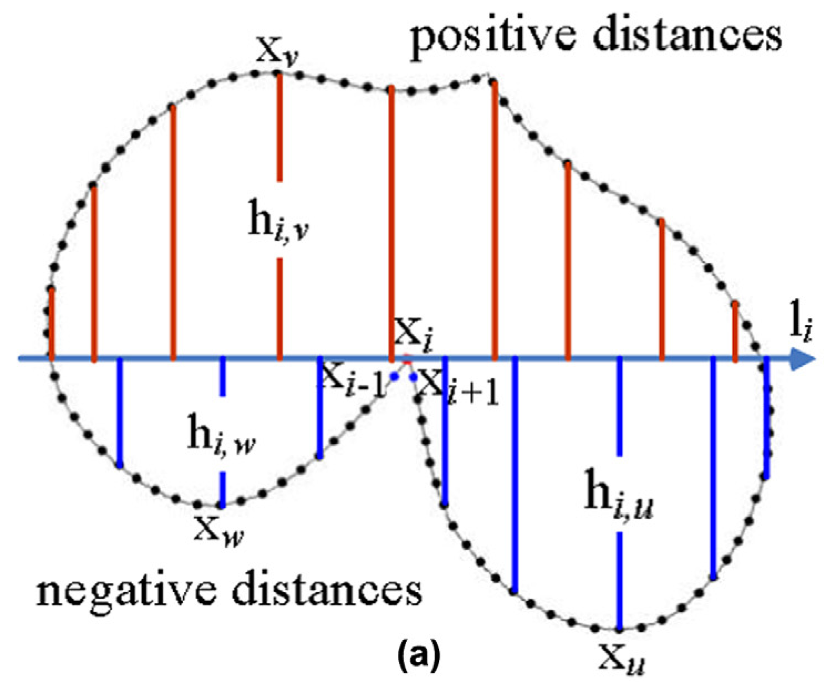
\includegraphics[width=0.7\textwidth]{figures/LitreatureReview/heightfunc.png}
        \caption[Example of height functions.]{(a) Example of height functions being calculated according to sample point $x_{i}$. Adapted from \cite{wang}.}
        \label{fig:heightfunc}
\end{figure*}

In Fig. \ref{fig:heightfunc}, the height functions for $x_{i}$ are being calculated. The tangent line $l{i}$ is defined by using $x_{i-1}$ and $x_{i+1}$. In this case, the tangent line is a horizontal one. Then the distance between other points and the tangent line is calculated. For instance, from point $x_{u}$ to tangent line $l_{i}$, the height value is $h_{i,u}$. Upon doing so we can determine on which side of the tangent line the calculated points lie. For instance $h_{i,y}$ has a positive value and therefore its corresponding point,$x_{y}$,lies to the left of the tangent line, while $h_{i,w}$ and $h_{i,u}$ have negative values therefore points $x_{u}$ and $x_{w}$ lie on the right of the tangent line. This is done for each of the sample points, their height value is calculated according to tangent line $l_{i}$. And the shape descriptor for point $x_{i}$ with respective to the shape X is the ordered sequence of the height values. \\

The development of efficient and robust shape descriptors is a topic of on going research. Apart from the ones described in this section are various other techniques have been developed \cite{descriptor1,descriptor2,descriptor3,descriptor4,descriptor5}.

\section{COSFIRE Filters}
COSFIRE filters are effective for key point detection and pattern recognition. They are trainable because they can be configured with any given prototypes. They are constructed by a configuration process which automatically analyses the dominant orientations and their mutual spatial arrangement of a given prototype pattern of interest \cite{Azzopardi_Petkov_2012}. We use Gabor filters to detect the dominant orientations. The response of a COSFIRE filter is computed as the weighted geometric mean of the involved Gabor filter responses. This means that a response is only achieved when all the concerned contour parts are present \cite{Azzopardi_Petkov_2012}.

\subsubsection {Gabor Filters}
A one dimensional Gabor function is defined as the multiplication of a sinusoid with a Gaussian window as shown Fig. \ref{fig:1DGabor}. Gabor functions have then been extended to two-dimensions, as the product of an elliptical Gaussian and a sinusoid plane wave \cite{Daugman1985}. Fig. \ref{fig:2DGabor} illustrates a Gabor function map that is tuned for vertical bars.

\begin{figure*}[h]
        \centering
        \begin{subfigure}[b]{0.3\textwidth}
                \centering
                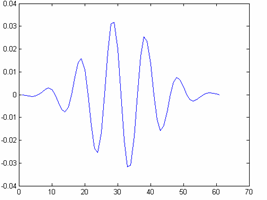
\includegraphics[width=1.0\textwidth]{figures/LitreatureReview/GaborFunction.png}
                \caption{Gabor Function}
                \label{fig:gabor}
        \end{subfigure}
        \begin{subfigure}[b]{0.3\textwidth}
                \centering
                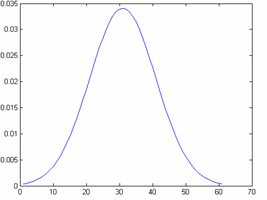
\includegraphics[width=1.0\textwidth]{figures/LitreatureReview/GaussianFunction.png}
                \caption{Gaussian Function}
                \label{fig:gaus}
        \end{subfigure}
        \begin{subfigure}[b]{0.3\textwidth}
                \centering
                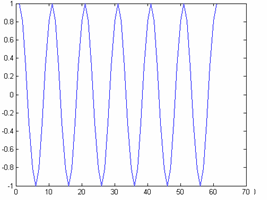
\includegraphics[width=1.0\textwidth]{figures/LitreatureReview/CosineFunction.png}
                \caption{Cosine Function}
                \label{fig:gaus}
        \end{subfigure}
        \caption[Example of a 1D Gabor Function]{(a) A one dimensional Gabor function is the product of a (b) Gaussian function and a (c) cosine function.}
        \label{fig:1DGabor}
\end{figure*}

\begin{figure*}[h]
        \centering
        \begin{subfigure}[b]{0.3\textwidth}
                \centering
                
\includegraphics[width=1.0\textwidth]{figures/LitreatureReview/GaborFunction2D.png}
                \caption{Gabor Function}
                \label{fig:gabor}
        \end{subfigure}
        \begin{subfigure}[b]{0.3\textwidth}
                \centering
                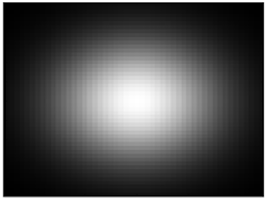
\includegraphics[width=1.0\textwidth]{figures/LitreatureReview/GaussianFunction2D.png}
                \caption{Gaussian Function}
                \label{fig:gaus}
        \end{subfigure}
        \begin{subfigure}[b]{0.3\textwidth}
                \centering
                
\includegraphics[width=1.0\textwidth]{figures/LitreatureReview/CosineFunction2D.png}
                \caption{Cosine Function}
                \label{fig:gaus}
        \end{subfigure}
        \caption[Example of a 2D Gabor Function]{(a) A two dimensional Gabor function is the product of an (b) elliptical Gaussian and a (c) complex plane wave.}
        \label{fig:2DGabor}
\end{figure*}

In their research Jones and Palmer \cite{JonesPalmer1987} demonstrated that two dimensional (2D) Gabor functions, which were proposed by Daugman \cite{Daugman1985}, can be used to model receptive fields of the orientation- selective simple cells of cats. Fig. \ref{fig:CatReceptiveField} shows the similarity between two dimensional Gabor functions and receptive fields of cats’ simple cells. The top row shows 2D receptive field profiles while the second row shows their corresponding best fitting Gabor functions \cite{Daugman1988}. \\


Daugman’s research \cite{Daugman1985} enabled the use of Gabor functions in computer vision applications as means to analyse images \cite{Daugman1988}. Recently, a novel CORF (Combination of Receptive Fields) computational model was proposed in \cite{CORF_2012}. The authors demonstrated that the CORF model exhibits more properties that are typical of simple cells than the Gabor function model. The CORF model also achieves better performance in contour detection tasks.


\begin{figure}[t]
        \centering
        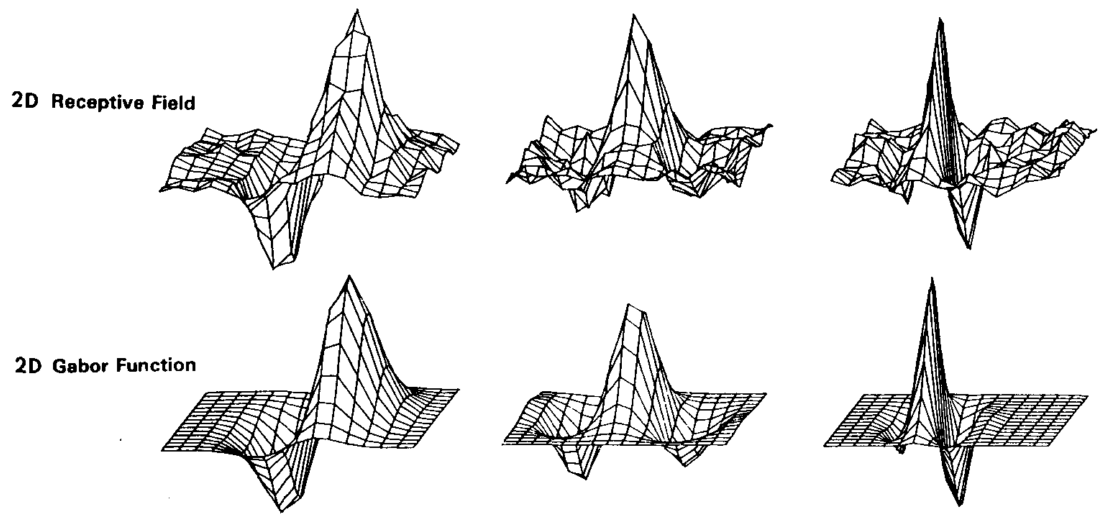
\includegraphics[width=1\textwidth]{figures/LitreatureReview/CatReceptiveFields.png}
        \caption[Receptive field profiles of some cells in cats visual cortex]{(First row) The receptive field profiles of some cells in a cat’s visual cortex compared to their corresponding best fitting (second row) two dimensional Gabor functions. Adapted from \cite{Daugman1988}.}
        \label{fig:CatReceptiveField}
\end{figure}




% Methods Chapter
\chapter{Methods}

% ============================================ OVERVIEW ===============================================
\section {Overview}
\label{sec:overview}

\subsection{The COSFIRE Approach}
COSFIRE filters are effective for keypoint detection and for pattern recognition. They are trainable because they can be configured with any given prototype patterns. They are constructed by a configuration process which automatically analyses the dominant orientations and their mutual spatial arrangement of a given prototype pattern of interest \cite{Azzopardi_Petkov_2012}. Gabor filters are used to detect the dominant orientations. The response of a COSFIRE filter is computed as the weighted geometric mean of the involved Gabor filter responses. This means that a response is only achieved when all the concerned contour parts are present \cite{Azzopardi_Petkov_2012}.


\subsection{Evaluation}
The research method applied in this project is quantitative. This also includes data analysis and hypothesis testing. Through the application of COSFIRE filters and classification techniques on publicly available data sets the performance measurements are computed in the form of true positives and false positive rates which are used to derive accuracy, precision and recall rates. The data sets that are used have different levels of complexity due to noise, deformation, rotation and scaling. The way we evaluate COSFIRE filters for these data set is as follows. \\

First, in a configuration stage, the COSFIRE filter is applied for each symbol model in the data set to create a collection of COSFIRE operators. Subsequently, with the attained COSFIRE operators, a shape descriptor is formed which takes an image as input and creates a feature vector representing the input image according to the operators from the configuration phase. Finally we use the resulting feature vectors to classify test images. \\


% ===================================================COSFIRE OVERVIEW================================================
\section {COSFIRE Method}
\label{sec:cosfiremethod}

\subsection{Overview}
COSFIRE filters are configured by first specifying a point of interest. In Fig.\ref{fig:ProtoTypePatternExample} a model symbol is used as an input image from which a local contour pattern is chosen as a prototype, encircled in Fig. \ref{fig:examplesymbol}. This prototype pattern is used to automatically configure a COSFIRE filter that responds to similar patterns.\\

\begin{figure*}[h]
        \centering
        \begin{subfigure}[b]{0.36\textwidth}
                \centering
                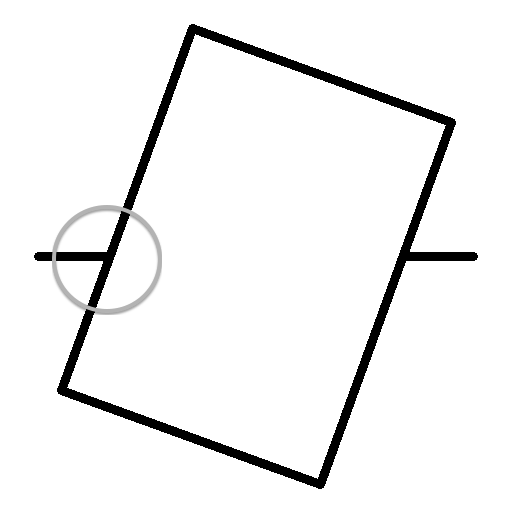
\includegraphics[width=0.6\textwidth]{figures/Method/ModelPointOfInterest.png}
                \caption{}
                \label{fig:examplesymbol}
        \end{subfigure}
        \begin{subfigure}[b]{0.36\textwidth}
                \centering
                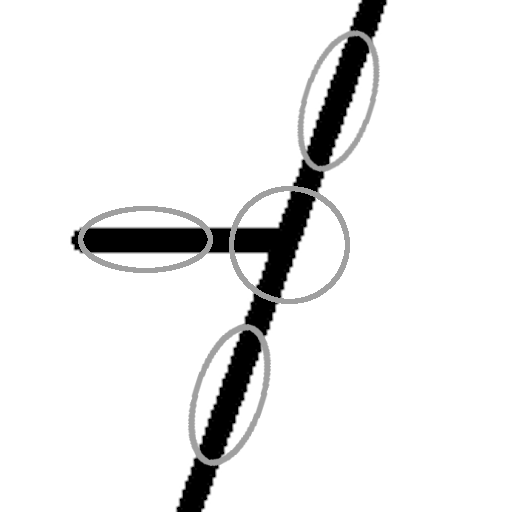
\includegraphics[width=0.6\textwidth]{figures/Method/DominantOrientationsAroundPointOfInterest.png}
                \caption{}
                \label{fig:modelsymbolvertex}
        \end{subfigure}
        \caption[Example of a prototype pattern]{(a) A model symbol (of size 512x512 pixels), of which one bifurcation (encircled) is used as a prototype pattern. (b) The enlarged prototype pattern where the dominant orientations around the point of interest are marked by 3 ellipses.}
        \label{fig:ProtoTypePatternExample}
\end{figure*}

The three ellipses shown in Fig. \ref{fig:modelsymbolvertex} around the encircled bifurcation illustrate the dominant orientations in the spatial arrangement around the chosen point of interest. These dominant orientations are detected by using symmetric Gabor filters. The selection of Gabor filter responses depends on the analysis of the local prototype pattern. The encircled bifurcation represents the overlapping support of a group of Gabor filters.

During the application of the COSFIRE method, different Gabor filter responses are taken at different locations around a point by shifting the responses of these Gabor filters by different vectors. The type of Gabor filters, the locations at which we take their responses, and the shifting vectors are determined in a automatic configuration stage. Then the shifted responses are used for the pixel-wise evaluation of a multivariate function which ultimately produces the COSFIRE filter's output.The COSFIRE filter achieves a response only when presented with the same or similar spatial arrangement of lines with similar orientations and thicknesses to the prototype.



% ======================================================GABOR FILTERS================================================
\subsection{Using Gabor filters to Detect Orientations}
The dominant orientations around a specified point of interest are detected by using symmetric two-dimensional (2D) Gabor filters. A 2D Gabor filter is defined as the product of an elliptical Gaussian and a sinusoid plane wave and is defined as follows:

\begin{equation}
   g(x,y;\lambda,\theta,\psi,\delta,\gamma) = \exp(-\frac{x'^2+\gamma^2y'^2}{2\delta^2}) \exp(2\pi \frac{x'}{\lambda}+\psi)
\end{equation}

\begin{equation}
x' = x \cos(\theta)+y\sin(\theta)
\end{equation}

\begin{equation}
y' = -x \sin(\theta)+y\cos(\theta)
\end{equation}

The $\lambda$ parameter, whose value is specified in pixels, represents the wavelength of the cosine factor, therefore the preferred wavelength of the filter. The $\theta$ parameter, who's value is specified in degrees, represents the orientation. The $\psi$ parameter represents the phase offset of the cosine factor whose values, from 0 to 180, determine whether the Gabor function is symmetric or not. A symmetric Gabor function is produced by setting the $\psi$,phase offset, parameter value to 0$^{\circ}$ or 180$^{\circ}$.\\

In this dissertation, the response of a symmetric Gabor filter at a given location (x,y) that is selective for a bar structure of orientation $\theta^{\circ}$ and thickness $2\lambda$ is denoted by $g_{\lambda,\theta}(x,y)$. The response represents the detection of a contour part within the image of wavelength $\lambda$ and of orientation $\theta^{\circ}$. Fig.\ref{fig:ModelGabor} shows two examples of Gabor filters, of the same wavelength but with different orientations being applied to a symbol model image. \\

\begin{figure*}[h]
        \centering
        \begin{subfigure}[b]{0.3\textwidth}
                \centering
                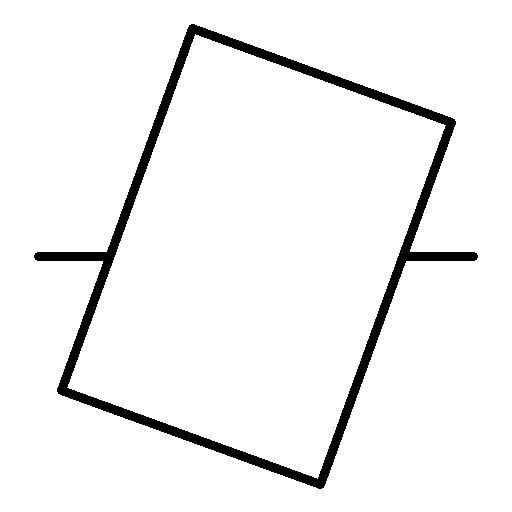
\includegraphics[width=0.8\textwidth]{figures/Method/ModelSymbol1.png}
                \caption{}
                \label{fig:examplesymbol2}
        \end{subfigure}
        \begin{subfigure}[b]{0.3\textwidth}
                \centering
                
\includegraphics[width=0.8\textwidth]{figures/Method/gabor_15_95.png}
                \caption{}
                \label{fig:gab1090}
        \end{subfigure}
        \begin{subfigure}[b]{0.3\textwidth}
                \centering
                
\includegraphics[width=0.8\textwidth]{figures/Method/gabor1_15_160.png}
                \caption{}
                \label{fig:gab10130}
        \end{subfigure} 
        \caption[Gabor filter applications]{(b) A Gabor filter when applied to a (a) model symbol with $\lambda = 15 $ and $\theta = 90^{\circ}$. (c) The response of a Gabor filter when applied to a (a) model symbol with $\lambda = 15 $ and $\theta = 160^{\circ}$.}
        \label{fig:ModelGabor}
\end{figure*}


We then threshold the Gabor responses in order to eliminate undesirable responses to some noise or to undesirable responses around the contour parts. This threshold, $t1 = (0 \leq t1 \leq 1)$, is a fraction of the maximum response of $g_{\lambda,\theta}(x,y)$ across all combinations of values $(\lambda,\theta)$ and all possible positions within the image $(x,y)$. The threshold responses are then denoted by $| g_{\lambda,\theta}(x,y)|_{t1}$. The value of the $t1$ threshold depends on the contrast the image contains. Ultimately, this threshold parameter controls the level at which a Gabor filter's response recognises the presence of a contour part. For our experiments we found that a value of t1 = 0.1 is sufficient.\\


% =============================================COSFIRE CONFIGURATION================================================
\subsection{Configuration}
As input, COSFIRE filters use the responses of specific Gabor filters. Each of these Gabor filters responses represent a contour part in an image. Each response is denoted as a set of four parameter values, $( \lambda_{i}, \theta_{i}, \rho_{i}, \phi_{i} )$. The width of the detected contour part is represented by $\lambda_{i}$. The orientation of the same contour part is represented by $\theta_{i}$. Finally its location is represented by polar coordinates $\rho_{i}$ and $\phi_{i}$ with respect to the point of interest.\\

The parameter values of these contour parts are obtained as follows. A circle of radius $\rho$ is placed around the point of interest. Along this circle we consider the responses of a bank of Gabor filters. From all those Gabor filters' responses we only take those that have the maximum response across all filters, that is across all combinations of $(\lambda, \theta)$. These are chosen to be the dominant orientations around the point of interest. We then determine the polar coordinates of the chosen points, in respect to the center of the COSFIRE filter. \\

\begin{figure*}[h]
        \centering
        \begin{subfigure}[b]{0.3\textwidth}
                \centering
                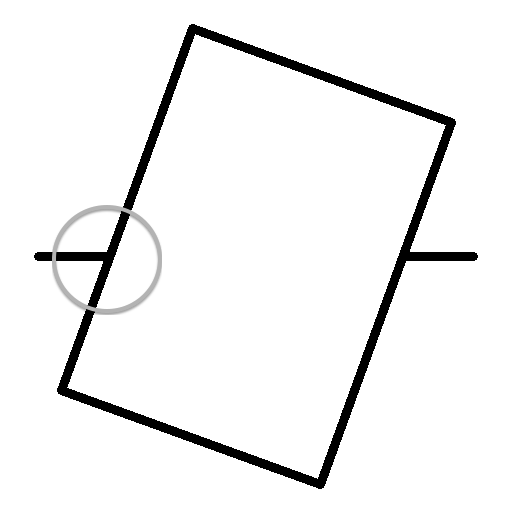
\includegraphics[width=0.8\textwidth]{figures/Method/ModelPointOfInterest.png}
                \caption{}
                \label{fig:modelsymbol}
        \end{subfigure}
        \begin{subfigure}[b]{0.3\textwidth}
                \centering
                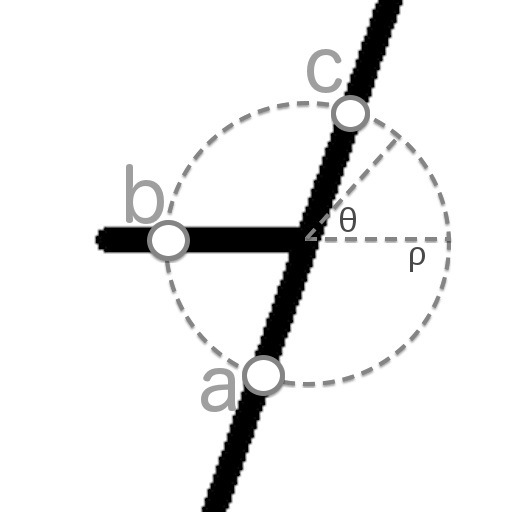
\includegraphics[width=0.8\textwidth]{figures/Method/actualConfiguration.jpg}
                \caption{}
                \label{fig:cosfireconf}
        \end{subfigure}
        \caption[Example configuration of a COSFIRE filter]{(a) A circle of radius $\rho$ is placed around a point of interest. (b) The points marked by labels a, b, and c represent the locations at which the Gabor filters achieve local maxima responses.}
        \label{fig:COSFIREConfigurationExample}
\end{figure*}


Fig. \ref{fig:COSFIREConfigurationExample} shows an example configuration of a COSFIRE filter by with a circle around the point of interest in a symbol model image. For each location ($\rho,\phi$) we then consider all the combinations of $(\lambda, \theta)$ for which the corresponding Gabor filter response, $_{g\lambda,\theta}(x,y)$, is greater than a fraction,$t_{2}=0.75$, of the maximum response across all the combinations of $\lambda$ and $\theta$.
For each value of $\theta$ that satisfies the condition above, we consider a single value of $\lambda$ from the maximum of all responses. For each unique pair of ($\lambda, \theta$), for location ($\rho,\phi$) we then obtain a tuple $( \lambda_{i}, \theta_{i}, \rho_{i}, \phi_{i} )$. \\

More than one tuple can also be formed in the same location. Therefore, we express the set of parameter value combinations as $S_f= \begin{Bmatrix}( \lambda_{i}, \theta_{i}, \rho_{i}, \phi_{i} ) | i=1...n_{f} \end{Bmatrix}$. The $f$ subscript stands for the local prototype pattern around the specified point of interest. Fig. \ref{fig:COSFIREConfigurationExample2} is an example of the resultant configured operator from Fig. \ref{fig:COSFIREConfigurationExample}.

\begin{figure*}[h]
        \centering
        \begin{subfigure}[b]{0.3\textwidth}
                \centering
                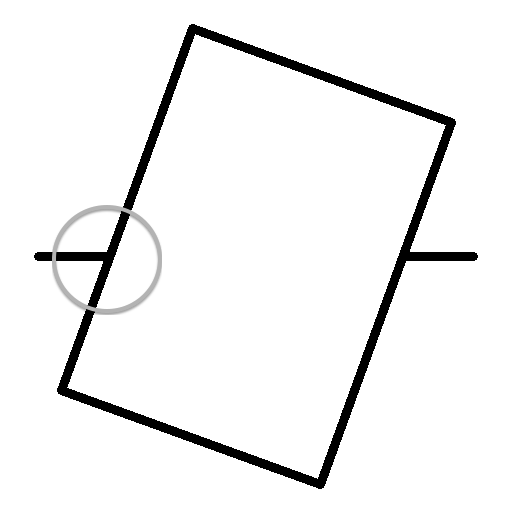
\includegraphics[width=0.8\textwidth]{figures/Method/ModelPointOfInterest.png}
                \caption{}
                \label{fig:modelsymbol}
        \end{subfigure}
        \begin{subfigure}[b]{0.3\textwidth}
                \centering
                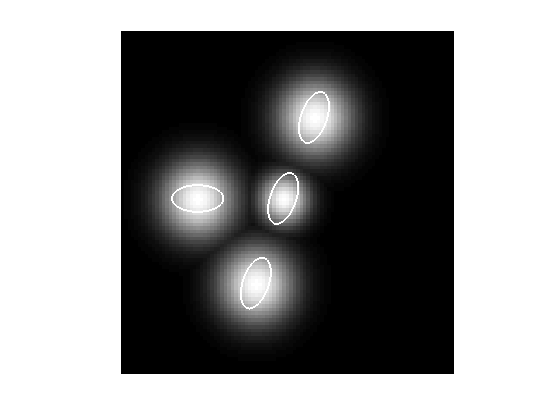
\includegraphics[width=0.8\textwidth]{figures/Method/COSFIREOPerator.png}
                \caption{}
                \label{fig:cosfireconf}
        \end{subfigure}
        \caption[Example of a COSFIRE operator for a prototype pattern.]{(b) A COSFIRE operator is configured upon selecting (a) a prototype pattern where $\rho = 14$ }
        \label{fig:COSFIREConfigurationExample2}
\end{figure*}

The following shows the collection of tuples,$S_{f}$, returned by the COSFIRE operator shown in Fig.\ref{fig:COSFIREConfigurationExample2}. These tuples are then used in the application of the COSFIRE filter.

\begin{equation}
  S_{f} = \begin{Bmatrix*} 
                  (\lambda_1 = 11.3137, & \theta_1 = 2.7925,    & \rho_1 = 0,  & \phi_1 = 0), \\
                  (\lambda_2 = 11.3137, & \theta_2 = 2.7925,    & \rho_2 = 14, &\phi_2 = 1.2043), \\
                  (\lambda_3 = 11.3137, & \theta_3 = 1.5708,    & \rho_3 = 14, &\phi_3 = 3.1416), \\
                  (\lambda_4 = 11.3137, & \theta_4 = 1.6581,    & \rho_4 = 14, &\phi_4 = 3.1416), \\
                  (\lambda_5 = 11.3137, & \theta_5 = 2.7925,    & \rho_5 = 14, &\phi_5 = 4.4157), \\
              \end{Bmatrix*}
\end{equation} \\

\subsection{Application of a COSFIRE Filter}
\subsubsection{Applying Gabor filters}
For each tuple $i$ in the configured set $S_f$ we apply a Gabor filter, to a test image, with the corresponding parameters $\lambda_i$ and $\theta_i$. A maximum response is achieved for a bar structure that has an orientation $\theta_i$ and thickness $2\lambda_i.$ 

\subsubsection{Blurring and Shifting of Gabor responses}
First, we blur the Gabor filter responses in order to allow for some tolerance in the position of their respective contour parts. \\

The blurring operation is defined as the computation of maximum value of the weighted thresholded responses of a Gabor filter. A Gaussian function, $G_{\sigma}(x,y)$, is used for weighting. The $\sigma$ parameter represents the standard deviation of the Gaussian function which is expressed as a linear function of distance $\rho$ from the center of the COSFIRE filter as shown in Eq. 1.5. where $\sigma_{0}$ and $\alpha$ are constants and the $\alpha$ parameter value determines the orientation tuning of the COSFIRE filter.

\begin{equation}
 \sigma = \sigma_{0}+\alpha\rho
\end{equation}
\label{eq:gStandardDeviation}

We then take the blurred Gabor filter responses and shift them to the filter's centre so they meet at the same position, the same position we consider the center of support of the concerned COSFIRE filter. Each response is shifted by a distance $\rho_{i}$ in the direction opposite of $\phi_{i}$. In polar coordinates the shift vector by which the Gabor filter responses are shifted is specified by $(\rho_{i},\phi_{i} + \pi)$ where as in cartesian coordinates it is specified as $(\Delta x_{i},\Delta y_{i})$ where $\Delta x_{i}=-\rho_{i} \cos(\phi_{i})$ and $\Delta y_{i}=-\rho_{i} \sin(\phi_{i})$. The blurred and shifted response of a Gabor filter, specified by the $i$-th tuple $( \lambda_{i}, \theta_{i}, \rho_{i}, \phi_{i} )$ in $S_{f}$, is denoted by $s_{( \lambda_{i}, \theta_{i}, \rho_{i}, \phi_{i} )}(x,y)$.

\begin{equation}
s_{( \lambda_{i}, \theta_{i}, \rho_{i}, \phi_{i} )}(x,y) = \underset{x',y'}{max} \begin{Bmatrix*} |g_{\lambda_{i}, \theta_{i}} (x-x'-\Delta x_{i},y-y'-\Delta y_{i})|_{t_{1}} G_{\sigma}(x',y') \end{Bmatrix*}
\end{equation}

\begin{equation}
-3\sigma \leq x,y \leq 3\sigma
\end{equation}



\subsubsection{Response of a COSFIRE filter}
The response of a COSFIRE filter, denoted by $r_{S_{f}}(x,y)$, is defined as the weighted geometric mean of all the thresholded blurred and shifted Gabor filter responses, denoted by $s_{\lambda_{i}, \theta_{i}, \rho_{i}, \phi_{i}} (x,y)$, that correspond to the contour parts defined in $S_{f}$: 


\begin{equation}
r_{S_{f}}(x,y) = \left|\left(\prod_{i=1}^{|S_{f}|} \left(s_{\lambda_{i}, \theta_{i}, \rho_{i}, \phi_{i}}(x,y)\right)^{\omega_{i}}\right)^{1/\sum_{i=1}^{|S_{f}|} \omega_{i}}\right|_{t_{3}}
\end{equation}

\begin{equation}
\omega_{i} = exp -\frac{\rho_{i}^2}{2\sigma'^2} , 0 \leq t_{3} \leq 1
\end{equation}

The $|.|_{t_{3}}$ stands for the thresholding the response at a fraction $t_{3}$ of its maximum across all image coordinates. COSFIRE filters can achieve invariance to rotation, scale, reflection and contrast inversion. We refer to \cite{Azzopardi_Petkov_2012} for the technical description of how invariance of COSFIRE filters is achieved


\section {Evaluation}
\label{sec:evaluation}
\subsection{Pre-Processing}
Each dataset's collection of test images varies according to some amount of deformation, noise or geometrical transformation. In order to aid the classification process a number of pre-processing steps were taken in order to clean/enhance the test images. As an initial step all test images are resized by a specific factor. 
Furthermore, test images which contain salt and pepper noise, such as noise E's, are de-noised using median filtering and degraded test images, such as Noise A's, are enhanced by the use of dilation. Other test images, such as Noise B's were thickened. Also with this thickening noise was included, therefore both median filtering and thinning were applied. The following are the pre-processing techniques which were applied in this evaluation.

\subsubsection{Re-sizing}
For efficiency reasons, prior to configuring COSFIRE filter/s we first resize the model by a factor of $0.5$, using bicubic interpolation, before being inputted into the configuration and training phases. The original model images are of size $(512 \times 512)$ pixels. By applying a resize factor of $0.5$, the images are resized to $(512(0.5) \times 512(0.5)) = (256 \times 256)$ pixels. This reduces the time in which the COSFIRE operator is applied to an image by half due to less information to process. No pre-processing was done on the test images.

\subsubsection{De-noising by median filtering}
Datasets such as the Noise E contain "salt and pepper" noise. Therefore before running an experiment using those datasets some pre-processing is required in order to reduce noise. De-noising is done through the use of median filtering. A median filter considers each pixel in the image sequentially and analyses the surrounding pixels. The value of the considered pixel is replaced with the median of the values of the surrounding pixels \cite{medianFiltering}. This reduces the noise from the image as shown in Fig. \ref{fig:mf} .

\begin{figure*}[h]
        \centering
        \begin{subfigure}[b]{0.3\textwidth}
                \centering
                \fbox{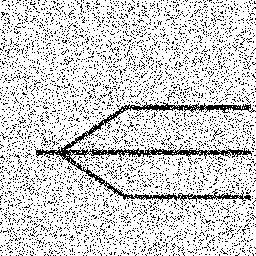
\includegraphics[width=0.8\textwidth]{figures/Method/image04.png}}
                \caption{}
                \label{fig:modelsymbol}
        \end{subfigure}
        \begin{subfigure}[b]{0.3\textwidth}
                \centering
                \fbox{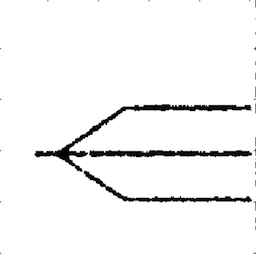
\includegraphics[width=0.8\textwidth]{figures/Method/untitled.png}}
                \caption{}
                \label{fig:mf123}
        \end{subfigure}
        \caption[Example output of median filtering.]{(a) A symbol with salt and pepper noise is (b) processed through the use of median filtering}
        \label{fig:mf}
\end{figure*}

\vspace{100mm}

\subsubsection{Dilation}
Some datasets, such as Noise A, have degraded test images. Before classifying such as test images an other pre-processing step that is implemented is morphological dilation. 
The effect of morphological dilation is to gradually enlarge the boundaries of specific regions of foreground pixels. Therefore these regions grow in size while holes or gaps within the symbol become smaller, thus enhancing the image. In order to do this a structuring element is used which determines the dilation effect on the test image \cite{dilation}. Fig \ref{fig:dilate} shows an example.

\begin{figure*}[h]
        \centering
        \begin{subfigure}[b]{0.3\textwidth}
                \centering
                \fbox{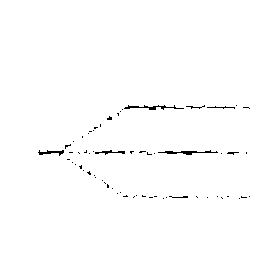
\includegraphics[width=0.8\textwidth]{figures/Method/image11.png}}
                \caption{}
                \label{fig:modelsymbol}
        \end{subfigure}
        \begin{subfigure}[b]{0.3\textwidth}
                \centering
                \fbox{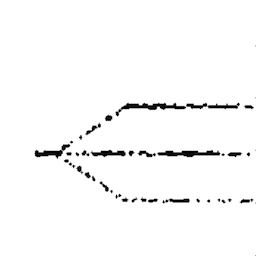
\includegraphics[width=0.8\textwidth]{figures/Method/image11Dilate.png}}
                \caption{}
                \label{fig:mf123}
        \end{subfigure}
        \caption[Example output of dilation.]{(a) A symbol of degraded quality (b) is processed using morphological dilation}
        \label{fig:dilate}
\end{figure*}

\subsubsection{Thinning}
Thinning is an other morphological operator which removes pixels so that an object shrinks to a minimal stroke. Like dilation, thinning relies on a structuring element \cite{thinning}. Datasets, such as noise B, contain test images which have their lines' thickened. Further more, the process of thickening the symbol's geometric parts adds noise around the edges as well. This is countered by doing the following. Like dilation, thinning relies on a structuring element \cite{thinning}. In this case, we use a structuring element of line form. Twelve different line structuring elements are created with different orientations. These orientations are applied to the test image and the outputs for each are then superimposed. Subsequently skeletonisation and dilation using a disc structuring elements are applied. A median filter is also applied, in order to remove the noise around the edges, and thinning. Fig \ref{fig:thickness} shows an example.

\begin{figure*}[h]
        \centering
        \begin{subfigure}[b]{0.3\textwidth}
                \centering
                \fbox{
\includegraphics[width=0.8\textwidth]{figures/Method/image03.png}}
                \caption{}
                \label{fig:modelsymbol}
        \end{subfigure}
        \begin{subfigure}[b]{0.3\textwidth}
                \centering
                \fbox{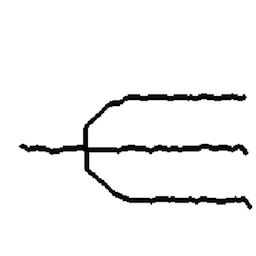
\includegraphics[width=0.8\textwidth]{figures/Method/image03Thinning.png}}
                \caption{}
                \label{fig:mf123}
        \end{subfigure}
        \caption[Example output of thinning.]{(a) A symbol of thickened quality (b) is processed using median filtering and thinning}
        \label{fig:thickness}
\end{figure*}

\subsection{Forming a Shape Descriptor}
\label{sec:descriptor}

In the configuration process of COSFIRE filters, features of interest are chosen by specifying a point or a collection of points within the model symbol. The system automatically analyses those points and extracts information about the dominant orientations and their mutual spatial arrangement according to the list of concentric circles surrounding the point of interest. The number of concentric circles is not intrinsic to the method but rather to the complexity of the given prototype pattern of interest. These are the prototype patterns that the COSFIRE filter will learn to recognise in the testing images. \cite{Azzopardi_Petkov_2012}. \\

For the purpose of electrical and architectural symbol recognition, a COSFIRE filter is configured for every model symbol in a given data set. These configurations were approached in two ways. In the first approach that was used in the first six experiments, was to select a single static point of interest which was placed in the middle of the model symbol. Fig. \ref{fig:COSFIREoperatorExample} shows a configuration, using the described single point approach.
%
\begin{figure*}[h]
        \centering
        \begin{subfigure}[b]{0.3\textwidth}
                \centering
                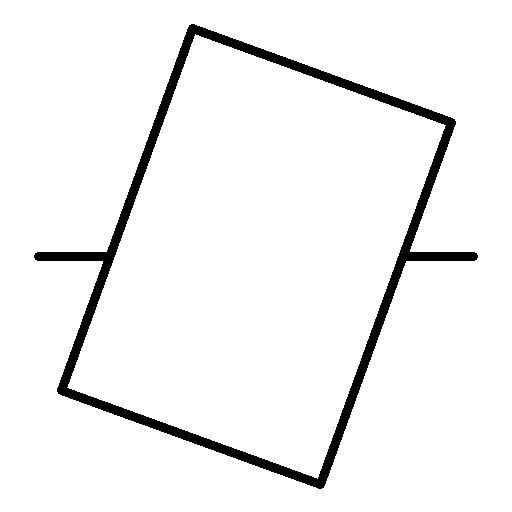
\includegraphics[width=0.8\textwidth]{figures/Method/ModelSymbol1.png}
                \caption{}
                \label{fig:modelsymbol}
        \end{subfigure}
        \begin{subfigure}[b]{0.3\textwidth}
                \centering
                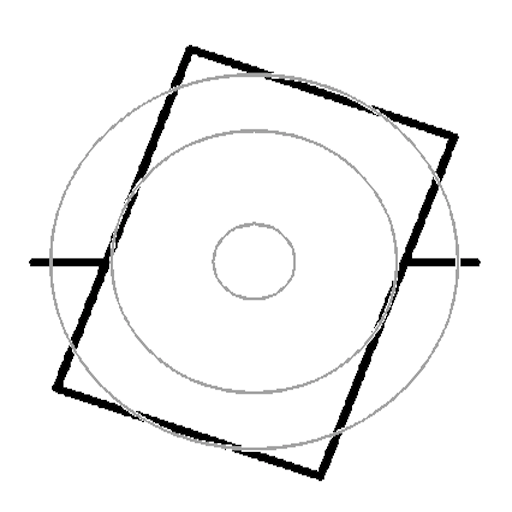
\includegraphics[width=0.8\textwidth]{figures/Method/ModelRhoConfiguration.png}
                \caption{}
                \label{fig:cosfireconf}
        \end{subfigure}
        \caption[Configuration of a COSFIRE filter using single point approach]{A COSFIRE filter is configured by first placing (b) the point of interest at the centre of the (a) model symbol}
        \label{fig:COSFIREoperatorExample}
\end{figure*}

The resulting COSFIRE filters are used to build a shape descriptor as follows. The created COSFIRE operators are applied to each symbol model. Each COSFIRE operator achieves a response for every location in the given image. From this response image, we choose the one that has the maximum value. This means that a symbol model image is described by a vector of values with a size that is equivalent to the number of COSFIRE filters used.\\

Fig. \ref{fig:shapedescriptor} shows an example of the result attained when the model symbols are processed by the shape descriptor. In this example there are 17 models images and 1 operator is applied to each model image. Each model image is therefore represented by a feature vector of 17 maximum values. The diagonal values in this descriptor have the highest responses. These values correspond to the model image being applied to it's corresponding COSFIRE operator.\\

\begin{figure*}[h]
    \centering
    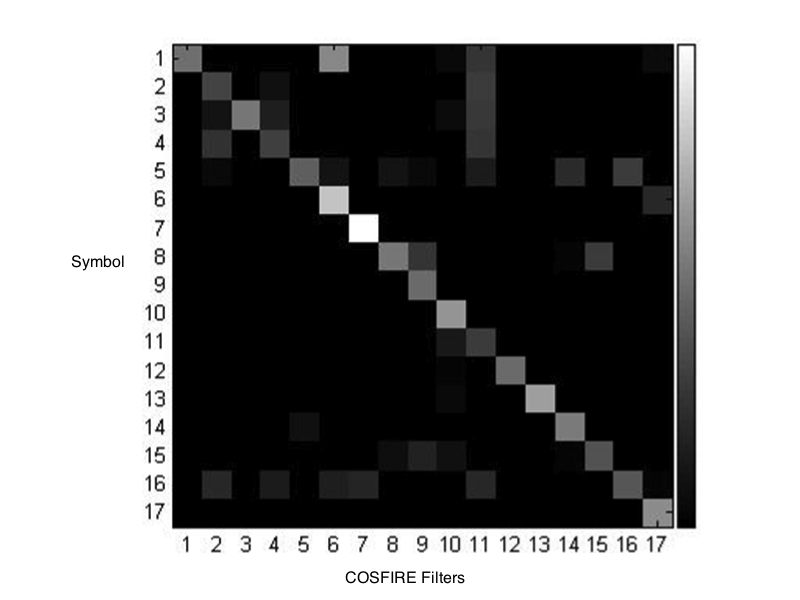
\includegraphics[totalheight=0.5\textheight, keepaspectratio]{figures/Method/ShapeDescriptor2.png}
    % \rule{.8\textwidth}{.8\textheight}{figures/ProjectPlan.jpg}
    \caption[Example of the feature vectors  for each model created by a shape descriptor]{A row {\em i} represents the feature vector of a symbol model composed of the maximum responses of COSFIRE filters. Element {\em j} of a feature vector {\em i} is the maximum response of a COSFIRE filter which is configured by model symbol {\em j}}
    \label{fig:shapedescriptor}
  \end{figure*}

Although the single point approach towards configuring filters produces good results in the first few datasets, a problem is introduced concerning the list of concentric circles used. Using the same list of concentric circles for all the datasets means that for some model symbols no dominant orientations could be detected.This resulted in test symbols not being properly recognised. An example is shown in Fig. \ref{fig:COSFIREoperatorErrorExample}.\\

\begin{figure*}[h]
        \centering
        \begin{subfigure}[b]{0.3\textwidth}
                \centering
                
\includegraphics[width=0.6\textwidth]{figures/Method/ModelSymbol2.png}
                \caption{Model Symbol}
                \label{fig:modelsymbol}
        \end{subfigure}
        \begin{subfigure}[b]{0.3\textwidth}
                \centering
                
\includegraphics[width=0.6\textwidth]{figures/Method/CosfireOperatorSinglePointApproachError.png}
                \caption{COSFIRE Operator}
                \label{fig:cosfireoperator}
        \end{subfigure}
        \caption[Example of an incorrect configuration due to rho list ]{(b) Inappropriate selection of concentric circles around the center of (a) a specific model symbol. Here we use the same three concentric circles used in the previous example.}
        \label{fig:COSFIREoperatorErrorExample}
\end{figure*}
%%
In order to address this issue, an alternative approach is taken in selecting points of interest. The list of concentric circles is set to three and three points of interest are placed randomly in the symbol model image. Each of these points hold the same list of concentric circles. Doing so ensures that each model symbol has a unique set of detected contour parts. An example of this approach is shown in Fig. \ref{fig:3PointCOSFIREoperatorExample}.

\begin{figure*}[h]
        \centering
        \begin{subfigure}[b]{0.4\textwidth}
                \centering
                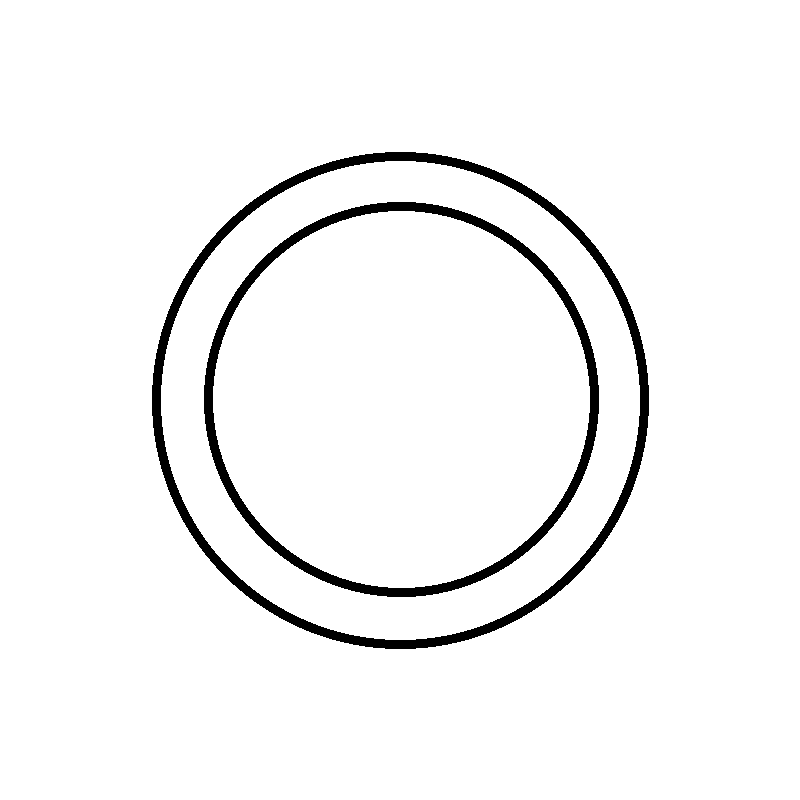
\includegraphics[width=0.8\textwidth]{figures/Method/ModelSymbol2_2.png}
                \caption{Model Symbol}
                \label{fig:modelsymbol}
        \end{subfigure}
        \begin{subfigure}[b]{0.4\textwidth}
                \centering
                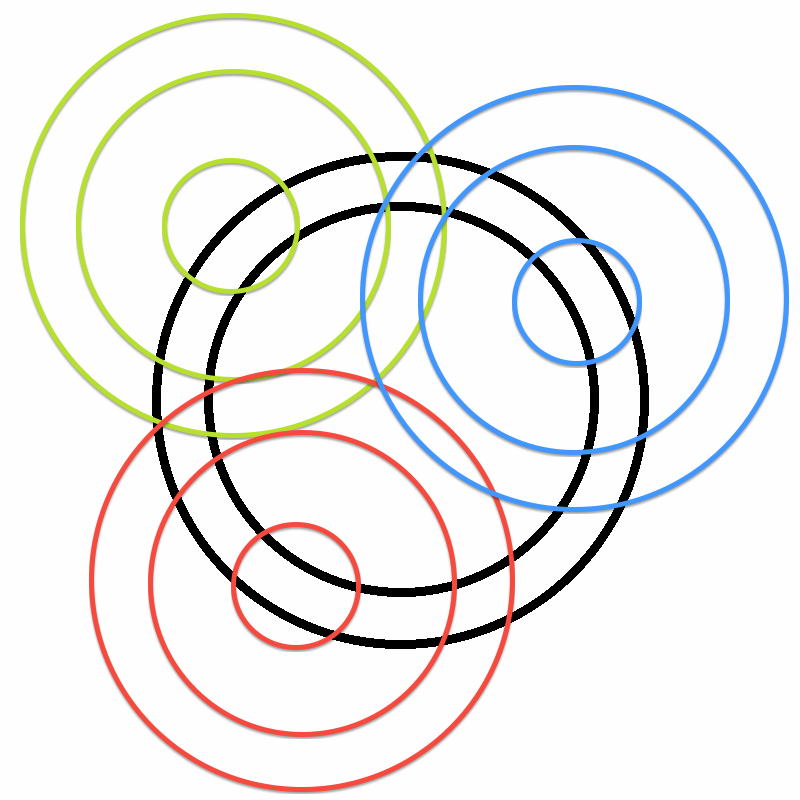
\includegraphics[width=0.8\textwidth]{figures/Method/CosfireOperatorThreePointApproach.png}
                \caption{COSFIRE Operator}
                \label{fig:cosfireoperator}
        \end{subfigure}
        \caption[An example of a 3-point approach in configuring COSFIRE filters.]{(b) Three COSFIRE filters are being configured for the symbol (a). The concentric circles for each point of interest are shown in different colours.}
        \label{fig:3PointCOSFIREoperatorExample}
\end{figure*}
\vspace{100mm}
This approach is driven by three parameters $\eta$, $\beta$, and $\varsigma$. The $\eta$ parameter value determines the number of points of interest placed in the model image. The $\beta$ parameter value determines the minimum number of tuples that should be attained from the point of interest's surrounding spatial arrangement. The $\varsigma$ parameter value determines the number of unique orientations that should be detected. This means that $\eta=3$ operators will be applied for each symbol mode. These operators should have a minimum of $\beta = 5$ tuples each with at least $\varsigma = 2$ unique orientations. \\

As a result of using the three point approach we have available a set of COSFIRE operators with a cardinality of three times the size of the total number of symbol model images available. Therefore for a dataset of $k$ model images, the configuration results in $3k$ distinct COSFIRE filter operators.
%[--!--]

%%============================================CLASSIFICATION===============================================
\subsection{Classification}
\label{sec:classify}
Classification refers to the problem of identifying, the set/s sets of categories/classes, certain objects or patterns belong to. In this thesis, this problem is tackled by trying to relate a test image to a specific symbol model by recognising contour parts which are similar in both the model image and the test image. This is done by using the feature vectors which represent both images.

\subsubsection{Feature Vectors}
Inputting each of the Model images into the shape descriptor, described in sub section \ref{sec:descriptor}, it creates a feature vector for each. This means that if there are 150 models in the data set and 3 operators are applied for each model 150 different feature vectors are created with 450 elements each. 

\subsubsection{Normalisation}
Prior to classification of the test images, normalisation is applied on both the training set of feature vectors and the testing set of feature vectors. This is done so that the test image and it's corresponding model image are rendered more comparable thus aiding the classification process. Normalisation is done using Z-Normalisation also known as zero-mean normalisation. This normalisation technique transforms the distribution of pixel values into a standard normal distribution. \\

For each 450 elements in the feature vector, the mean, $\mu_{x}$, and the standard deviation, $\sigma_{x}$, are computed. The configuration feature vectors are then normalised by subtracting the mean and diving the standard deviation. The same is done for the feature vectors which are extracted from the testing images. The following is how a normalised value is obtained using z-score normalisation \cite{zscore}:

\begin{equation}
 NormalisedValue = \frac{v-\mu_{x}}{\sigma_{x}}
\end{equation}
\label{eq:gStandardDeviation}


\subsubsection{K-nearest neighbour algorithm}
The K-nearest neighbour algorithm (K-nn), known to be amongst the top 10 data mining algorithms \cite{Wu_2007}, is a versatile technique who's application range from vision to computational geometry \cite{knn_online}. It has been used for the classification of objects or patterns according to the closest training examples available. Before using the Knn algorithm, some prerequisite steps need to be taken. The first step is to ensure that the data is in a feature space. This data can be both single scalars or even multidimensional vectors \cite{knn_online}. The second step is to define a constant $K$. \\

The constant $K$ is a user defined value. It is the number of instances / neighbours the algorithm allows to influence the classification \cite{knn_online}. Since the test symbol needs to be assigned to the class of its nearest neighbour, the constant $k$ is set to $k=1$. An other important step is to determine which distance metric to use. In order to classify the test image's feature vector to the nearest feature vector from the models a distance metric needs to be used. Since both the models and the test images are represented by feature vectors made of $n$ number of elements, the distance metric used in this classification process is Euclidean distance. Euclidean distance is defined as follows where $M$ is the feature vector for the model image and $T$ is the feature vector for the test image \cite{euclidean_online}. 

\begin{equation}
    d(M,T) = \sqrt{\sum_{i=1}^{n} (M_{i}-T)^2}
\end{equation}

Therefore classification is achieved by computing the Euclidean distance between the test image feature vector to each training feature vector in the shape descriptor. A test vector is then classified to the symbol for which the Euclidean distance is the smallest, therefore the most similar. An illustration of the Knn algorithm is shown in Fig. \ref{fig:knnexample}.


\begin{figure*}[h]
    \centering
    \includegraphics[totalheight=0.25\textheight, keepaspectratio]{figures/Method/knn.jpg}
    \caption[Example of K-nearest Neighbour algorithm]{An object (star) whose class is not known is being classified according to its nearest neighbours. Two examples are shown, where $k=3$ and $k=7$ \footnotemark.}
    \label{fig:knnexample}
\end{figure*}
\vspace{100mm}
\footnotetext[1]{Taken From \url{http://iopscience.iop.org/1742-5468/2010/11/P11015/fulltext/}}

.
\vspace{200mm}
\subsection{Evaluation Summary} 
Fig. \ref{fig:flowchart} shows a work flow of the whole evaluation process for this dissertation.
\begin{figure*}[h]
        \centering
        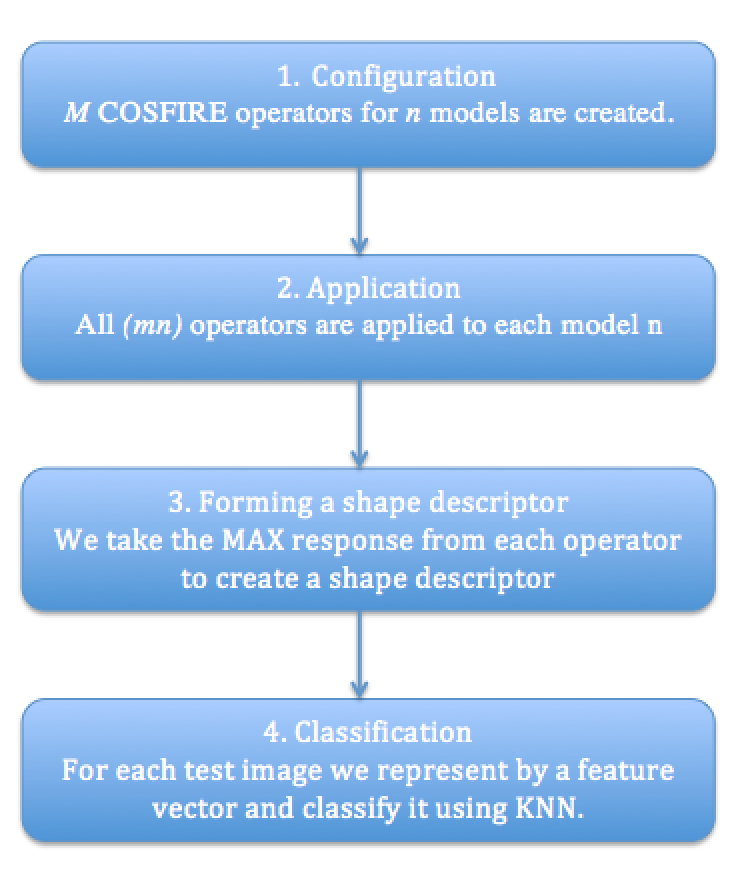
\includegraphics[width=0.8\textwidth]{figures/Method/workflow3.png}
        \caption[Evaluation flow chart]{(1) $M$ COSFIRE operators for $n$ model images are created. (2) All $(mn)$ operators are applied to each of the model images and (3) from those responses we take the maximum responses and create a feature vector for each model to form a shape descriptor. (4) We finally use the created shape descriptor to classify the images.  }
        \label{fig:flowchart}
\end{figure*}

% Results Chapter
\chapter{Experimental Results}
\section {Overview}
We start by evaluating the proposed method on the data set with the least level of complexity, category 1, which contains noiseless test images given in the same orientation and scale of their corresponding models. Then we apply the method to the data set with the second lowest complexity, categories 2 and 3, and finally we evaluate the COSFIRE filters on the data set with the highest level of complexity, category 4. The mentioned order in which  the experiments are run facilitates the analysis of the performance results and gives insight on further tuning the method. The following sub-sections are the results attained for each dataset.\\

\section {Category 1 Datasets}
\subsection{Sketches25f}
This sub category of datasets is split into three different sets namely Sketches25f-level1, Sketches25f-level2, and Sketches25f-level3. Each of these data sets consist of 17 different model symbols. These model symbols consist of straight lines only and do not include any arcs or circles. This data set holds 1000 test images. This test images are given in the same orientation and in the same scale of the models. However, these test images are deformed symbols of increasing complexity according to level. Fig.\ref{fig:Sketches25fExamples} illustrates a sample of this dataset.
    
    \begin{figure*}[h]
        \centering
                \begin{subfigure}[b]{0.2\textwidth}
                \centering
                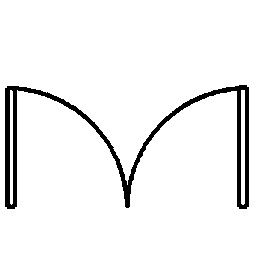
\includegraphics[width=0.73\textwidth]{figures/Results/Sketches25f/Model.png}
                \caption{Model}
        \end{subfigure}\\
                \begin{subfigure}[b]{0.25\textwidth}
                \centering
                
\includegraphics[width=0.9\textwidth]{figures/Results/Sketches25f/level1.png}
                \caption{Level 1}
        \end{subfigure}
                \begin{subfigure}[b]{0.25\textwidth}
                \centering
                \includegraphics[width=0.9\textwidth]{figures/Results/Sketches25f/level2.png}
                \caption{Level 2}
        \end{subfigure}
                \begin{subfigure}[b]{0.25\textwidth}
                \centering
                \includegraphics[width=0.9\textwidth]{figures/Results/Sketches25f/level3.png}
                \caption{Level 3}
        \end{subfigure}
        \caption[Sample data from 'Sketches25f' dataset]{Sample test images from the three different datasets under Sketches25f are shown for (a) a model symbol. (b) is a sample of Sketches25f-level1 , (c)  is a sample of Sketches25f-level2 and (d) is a sample of Sketches25f-level3.}
        \label{fig:Sketches25fExamples}
\end{figure*}

\subsubsection{Results}
\begin{table}[h]
\centering
\caption{Recognition results for dataset 'Sketches25f'}
\begin{tabular}{ccccccccccccccc}
  \hline
      Degradation Level & & & & & & & & Recognition Rate \\
  \hline
     1 & & & & & & & &  100 \% \\
     2 & & & & & & & &  100 \% \\
     3 & & & & & & & &  100 \% \\
  \hline
\end{tabular}
\end{table}



\vspace{85mm}

\subsection{Sketches25}
This sub category of datasets is split into three different sets namely Sketches25-level1, Sketches25-level2, and Sketches25-level3. Each of these data sets consist of 25 different model symbols. These model symbols consist of both straight lines and arcs or circles. This data set holds 1000 test images. This test images are given in the same orientation and in the same scale of the models. However, these test images are deformed symbols of increasing complexity according to level. Fig.\ref{fig:Sketches25Examples} illustrates a sample of this dataset.


    \begin{figure*}[h]
        \centering
                \begin{subfigure}[b]{0.2\textwidth}
                \centering
                \includegraphics[width=0.73\textwidth]{figures/Results/Sketches25/Model.png}
                \caption{Model}
        \end{subfigure}\\
                \begin{subfigure}[b]{0.25\textwidth}
                \centering
                \includegraphics[width=0.9\textwidth]{figures/Results/Sketches25/level1.png}
                \caption{Level 1}
        \end{subfigure}
                \begin{subfigure}[b]{0.25\textwidth}
                \centering
                \includegraphics[width=0.9\textwidth]{figures/Results/Sketches25/level2.png}
                \caption{Level 2}
        \end{subfigure}
                \begin{subfigure}[b]{0.25\textwidth}
                \centering
                \includegraphics[width=0.9\textwidth]{figures/Results/Sketches25/level3.png}
                \caption{Level 3}
        \end{subfigure}
        \caption[Sample data from 'Sketches25' dataset]{Sample test images from the three different datasets under Sketches25 are shown for (a) a model symbol. (b) is a sample of Sketches25-level1 , (c)  is a sample of Sketches25-level2 and (d) is a sample of Sketches25-level3.}
        \label{fig:Sketches25Examples}
\end{figure*}

\subsubsection{Results}
\begin{table}[H]
\centering
\caption{Recognition results for dataset 'Sketches25'}
\begin{tabular}{ccccccccccccccc}
  \hline
      Degradation Level & & & & & & & & Recognition Rate \\
  \hline
     1 & & & & & & & &  100 \% \\
     2 & & & & & & & &  100 \% \\
     3 & & & & & & & &  100 \% \\
  \hline
\end{tabular}
\end{table}

\vspace{49.3mm}

\subsection{Sketches50f}
This sub category of datasets is split into three different sets namely Sketches50f-level1, Sketches50f-level2, and Sketches50f-level3. Each of these data sets consist of 26 different model symbols. These model symbols consist of straight lines only and do not include any arcs or circles. This data set holds 1000 test images. This test images are given in the same orientation and in the same scale of the models. However, these test images are deformed symbols of increasing complexity according to level. Fig.\ref{fig:Sketches50fExamples} illustrates a sample of this dataset.

    \begin{figure*}[h]
        \centering
                \begin{subfigure}[b]{0.2\textwidth}
                \centering
                \includegraphics[width=0.73\textwidth]{figures/Results/Sketches50f/Model.png}
                \caption{Model}
        \end{subfigure}\\
                \begin{subfigure}[b]{0.25\textwidth}
                \centering
                \includegraphics[width=0.9\textwidth]{figures/Results/Sketches50f/level1.png}
                \caption{Level 1}
        \end{subfigure}
                \begin{subfigure}[b]{0.25\textwidth}
                \centering
                \includegraphics[width=0.9\textwidth]{figures/Results/Sketches50f/level2.png}
                \caption{Level 2}
        \end{subfigure}
                \begin{subfigure}[b]{0.25\textwidth}
                \centering
                \includegraphics[width=0.9\textwidth]{figures/Results/Sketches50f/level3.png}
                \caption{Level 3}
        \end{subfigure}
        \caption[Sample data from 'Sketches50f' dataset]{Sample test images from the three different datasets under Sketches50f are shown for (a) a model symbol. (b) is a sample of Sketches50f-level1 , (c)  is a sample of Sketches50f-level2 and (d) is a sample of Sketches50f-level3.}
        \label{fig:Sketches50fExamples}
\end{figure*}

\subsubsection{Results}
\begin{table}[H]
\centering
\caption{Recognition results for dataset 'Sketches50f'}
\begin{tabular}{ccccccccccccccc}
  \hline
     Degradation Level & & & & & & & & Recognition Rate \\
  \hline
     1 & & & & & & & &  100 \% \\
     2 & & & & & & & &  99.8 \% \\
     3 & & & & & & & &  99.4 \% \\

  \hline
\end{tabular}
\end{table}
\vspace{49.3mm}

\subsection{Sketches50}
This sub category of datasets is split into three different sets namely Sketches50-level1, Sketches50-level2, and Sketches50-level3. Each of these data sets consist of 50 different model symbols. These model symbols consist of both straight lines and arcs or circles. This data set holds 1000 test images. This test images are given in the same orientation and in the same scale of the models. However, these test images are deformed symbols of increasing complexity according to level. Fig.\ref{fig:Sketches50Examples} illustrates a sample of this dataset.

    \begin{figure*}[h]
        \centering
                \begin{subfigure}[b]{0.2\textwidth}
                \centering
                \includegraphics[width=0.73\textwidth]{figures/Results/Sketches50/Model.png} 
                \caption{Model}
        \end{subfigure}\\
                \begin{subfigure}[b]{0.25\textwidth}
                \centering
                \includegraphics[width=0.9\textwidth]{figures/Results/Sketches50/level1.png}
                \caption{Level 1}
        \end{subfigure}
                \begin{subfigure}[b]{0.25\textwidth}
                \centering
                \includegraphics[width=0.9\textwidth]{figures/Results/Sketches50/level2.png}
                \caption{Level 2}
        \end{subfigure}
                \begin{subfigure}[b]{0.25\textwidth}
                \centering
                \includegraphics[width=0.9\textwidth]{figures/Results/Sketches50/level3.png}
                \caption{Level 3}
        \end{subfigure}
        \caption[Sample data from 'Sketches50' dataset]{Sample test images from the three different datasets under Sketches50 are shown for (a) a model symbol. (b) is a sample of Sketches50-level1 , (c)  is a sample of Sketches50-level2 and (d) is a sample of Sketches50-level3.}
        \label{fig:Sketches50Examples}
\end{figure*}

\subsubsection{Results}
\begin{table}[H]
\centering
\caption{Recognition results for dataset 'Sketches50'}
\begin{tabular}{ccccccccccccccc}
  \hline
     Degradation Level & & & & & & & & Recognition Rate \\
  \hline
     1 & & & & & & & &  100 \% \\
     2 & & & & & & & &  100 \% \\
     3 & & & & & & & &  100 \% \\
  \hline
\end{tabular}
\end{table}

\vspace{49.3mm}

\subsection{Sketches100f}
This sub category of datasets is split into three different sets namely Sketches100f-level1, Sketches100f-level2, and Sketches100f-level3. Each of these data sets consist of 51 different model symbols. These model symbols consist of straight lines only and do not include any arcs or circles. This data set holds 1000 test images. This test images are given in the same orientation and in the same scale of the models. However, these test images are deformed symbols of increasing complexity according to level. Fig.\ref{fig:Sketches100fExamples} illustrates a sample of this dataset.

    \begin{figure*}[h]
        \centering
                \begin{subfigure}[b]{0.2\textwidth}
                \centering
                \includegraphics[width=0.73\textwidth]{figures/Results/Sketches100f/Model.png}
                \caption{Mode}
        \end{subfigure}\\
                \begin{subfigure}[b]{0.25\textwidth}
                \centering
                \includegraphics[width=0.9\textwidth]{figures/Results/Sketches100f/level1.png}
                \caption{level 1}
        \end{subfigure}
                \begin{subfigure}[b]{0.25\textwidth}
                \centering
                \includegraphics[width=0.9\textwidth]{figures/Results/Sketches100f/level2.png}
                \caption{level 2}
        \end{subfigure}
                \begin{subfigure}[b]{0.25\textwidth}
                \centering
                \includegraphics[width=0.9\textwidth]{figures/Results/Sketches100f/level3.png}
                \caption{level 3}
        \end{subfigure}
        \caption[Sample data from 'Sketches100f' dataset]{Sample test images from the three different datasets under Sketches100f are shown for (a) a model symbol. (b) is a sample of Sketches100f-level1 , (c)  is a sample of Sketches100f-level2 and (d) is a sample of Sketches100f-level3.}
        \label{fig:Sketches100fExamples}
\end{figure*}

\subsubsection{Results}
\begin{table}[H]
\centering
\caption{Recognition results for dataset 'Sketches100f'}
\begin{tabular}{ccccccccccccccc}
  \hline
      Degradation Level & & & & & & & & Recognition Rate \\
  \hline
     1 & & & & & & & &  98.1 \% \\
     2 & & & & & & & &  98.7 \% \\
     3 & & & & & & & &  98.1 \% \\

  \hline
\end{tabular}
\end{table}

\vspace{49.3mm}

\subsection{Sketches100}
This sub category of datasets is split into three different sets namely Sketches100-level1, Sketches100-level2, and Sketches500-level3. Each of these data sets consist of 100 different model symbols. These model symbols consist of both straight lines and arcs or circles. This data set holds 1000 test images. This test images are given in the same orientation and in the same scale of the models. However, these test images are deformed symbols of increasing complexity according to level. Fig.\ref{fig:Sketches100Examples} illustrates a sample of this dataset.

    \begin{figure*}[h]
        \centering
                \begin{subfigure}[b]{0.2\textwidth}
                \centering
                \includegraphics[width=0.73\textwidth]{figures/Results/Sketches100/Models.png}
                \caption{Model}
                \end{subfigure}\\
                \begin{subfigure}[b]{0.25\textwidth}
                \centering
                \includegraphics[width=0.9\textwidth]{figures/Results/Sketches100/level1.png}
                \caption{Level 1}
        \end{subfigure}
                \begin{subfigure}[b]{0.25\textwidth}
                \centering
                \includegraphics[width=0.9\textwidth]{figures/Results/Sketches100/level2.png}
                \caption{Level 2}
        \end{subfigure}
                \begin{subfigure}[b]{0.25\textwidth}
                \centering
                \includegraphics[width=0.9\textwidth]{figures/Results/Sketches100/level3.png}
                \caption{Level 3}
        \end{subfigure}
        \caption[Sample data from 'Sketches100' dataset]{Sample test images from the three different datasets under Sketches100 are shown for (a) a model symbol. (b) is a sample of Sketches100-level1 , (c)  is a sample of Sketches100-level2 and (d) is a sample of Sketches100-level3.}
        \label{fig:Sketches100Examples}
\end{figure*}

\subsubsection{Results}
\begin{table}[H]
\centering
\caption{Recognition results for dataset 'Sketches100'}
\begin{tabular}{ccccccccccccccc}
  \hline
     Degradation Level & & & & & & & & Recognition Rate \\
  \hline
     1 & & & & & & & &  99.2 \% \\
     2 & & & & & & & &  98.9 \% \\
     3 & & & & & & & &  98.2 \% \\

  \hline
\end{tabular}
\end{table}

\vspace{49.3mm}

\subsection{Sketches150f}
This sub category of datasets is split into three different sets namely Sketches150f-level1, Sketches150f-level2, and Sketches150f-level3. Each of these data sets consist of 80 different model symbols. These model symbols consist of straight lines only and do not include any arcs or circles. This data set holds 1000 test images. This test images are given in the same orientation and in the same scale of the models. However, these test images are deformed symbols of increasing complexity according to level. Fig.\ref{fig:Sketches150fExamples} illustrates a sample of this dataset.

    \begin{figure*}[h]
        \centering
                \begin{subfigure}[b]{0.2\textwidth}
                \centering
                \includegraphics[width=0.73\textwidth]{figures/Results/Sketches150f/Model.png}
                \caption{Model}
        \end{subfigure}\\
                \begin{subfigure}[b]{0.25\textwidth}
                \centering
                \includegraphics[width=0.9\textwidth]{figures/Results/Sketches150f/level1.png}
                \caption{Level 1}
        \end{subfigure}
                \begin{subfigure}[b]{0.25\textwidth}
                \centering
                \includegraphics[width=0.9\textwidth]{figures/Results/Sketches150f/level2.png}
                \caption{Level 2}
        \end{subfigure}
                \begin{subfigure}[b]{0.25\textwidth}
                \centering
                \includegraphics[width=0.9\textwidth]{figures/Results/Sketches150f/level3.png}
                \caption{Level 3}
        \end{subfigure}
        \caption[Sample data from 'Sketches150f' dataset]{Sample test images from the three different datasets under Sketches150f are shown for (a) a model symbol. (b) is a sample of Sketches150f-level1 , (c)  is a sample of Sketches150f-level2 and (d) is a sample of Sketches150f-level3.}
        \label{fig:Sketches150fExamples}
\end{figure*}


\subsubsection{Results}
\begin{table}[H]
\centering
\caption{Recognition results for dataset 'Sketches150f'}
\begin{tabular}{ccccccccccccccc}
  \hline
      Degradation Level & & & & & & & & Recognition Rate \\
  \hline
     1 & & & & & & & &  99.3 \% \\
     2 & & & & & & & &  99.2 \% \\
     3 & & & & & & & &  98.8 \% \\

  \hline
\end{tabular}
\end{table}
\vspace{49.3mm}

\subsection{Sketches150}
This sub category of datasets is split into three different sets namely Sketches150-level1, Sketches150-level2, and Sketches150-level3. Each of these data sets consist of 150 different model symbols. These model symbols consist of both straight lines and arcs or circles. This data set holds 1000 test images. These test images are given in the same orientation and in the same scale of the models. However, these test images are deformed symbols of increasing complexity according to level. Fig.\ref{fig:Sketches150Examples} illustrates a sample of this dataset.

    \begin{figure*}[h]
        \centering
                \begin{subfigure}[b]{0.2\textwidth}
                \centering
                \includegraphics[width=0.73\textwidth]{figures/Results/Sketches150/Model.png}
                \caption{Model}
        \end{subfigure}\\
                \begin{subfigure}[b]{0.25\textwidth}
                \centering
                \includegraphics[width=0.9\textwidth]{figures/Results/Sketches150/level1.png}
                \caption{Level 1}
        \end{subfigure}
                \begin{subfigure}[b]{0.25\textwidth}
                \centering
                \includegraphics[width=0.9\textwidth]{figures/Results/Sketches150/level2.png}
                \caption{Level 2}
        \end{subfigure}
                \begin{subfigure}[b]{0.25\textwidth}
                \centering
                \includegraphics[width=0.9\textwidth]{figures/Results/Sketches150/level3.png}
                \caption{Level 3}
        \end{subfigure}
        \caption[Sample data from 'Sketches150' dataset]{Sample test images from the three different datasets under Sketches150 are shown for (a) a model symbol. (b) is a sample of Sketches150-level1 , (c)  is a sample of Sketches150-level2 and (d) is a sample of Sketches150-level3.}
        \label{fig:Sketches150Examples}
\end{figure*}

\subsubsection{Results}
\begin{table}[H]
\centering
\caption{Recognition results for dataset 'Sketches150'}
\begin{tabular}{ccccccccccccccc}
  \hline
      Degradation Level & & & & & & & & Recognition Rate \\
  \hline
     1 & & & & & & & &  99.3 \% \\
     2 & & & & & & & &  98.9 \% \\
     3 & & & & & & & &  97.6 \% \\

  \hline
\end{tabular}
\end{table}
\vspace{49.3mm}


\section {Category 2 Datasets}
\subsection{Rotation}
This data set consists of 150 different models and 10 test symbols for each of those models.These model symbols consist of both straight lines and arcs or circles. In total this dataset holds 1500 test images. The test images are given in the same scale of the models. Orientation varies through out the 25 test symbols for each model. No noise is introduced to the test images. Fig. \ref{fig:RotationExamples} illustrates a few samples.

    \begin{figure*}[h]
    
        \centering
                \begin{subfigure}[b]{0.2\textwidth}
                \centering
                \includegraphics[width=0.81\textwidth]{figures/Results/Rotation/Model.png}
                \caption{}
        \end{subfigure}\\
                \begin{subfigure}[b]{0.25\textwidth}
                \centering
                \includegraphics[width=0.85\textwidth]{figures/Results/Rotation/1.png}
                \put(8,40){$\cdots$}
                \caption{}
        \end{subfigure}
        \qquad
                \begin{subfigure}[b]{0.25\textwidth}
                \centering
                \includegraphics[width=0.9\textwidth]{figures/Results/Rotation/2.png}
                \put(8,40){$\cdots$}
                \caption{}
        \end{subfigure}
        \qquad
                \begin{subfigure}[b]{0.25\textwidth}
                \centering
                \includegraphics[width=0.7\textwidth]{figures/Results/Rotation/3.png}
                \caption{}
        \end{subfigure}
        \caption[Sample data from the 'Rotation' dataset]{(b) (c) (d) Three test images for (a) a model symbol are illustrated from the Rotation dataset }
        \label{fig:RotationExamples}
\end{figure*}

\subsubsection{Results}
\begin{table}[H]
\centering
\caption{Recognition results for dataset 'Rotation'}
\begin{tabular}{ccccccccccccccc}
  \hline
      Recognition Rate \\
  \hline
      72.6 \% \\
  \hline
\end{tabular}
\end{table}
\vspace{85mm}

\subsection{Scaling}
This data set consists of 150 different models and 10 test symbols for each of those models.These model symbols consist of both straight lines and arcs or circles. In total this dataset holds 1500 test images. The test images are given in the same orientation of the models. Scaling varies through out the 25 test symbols for each model. No noise is introduced to the test images. Fig. \ref{fig:ScalingExamples} illustrates a few samples.

    \begin{figure*}[h]
        \centering
                \begin{subfigure}[b]{0.2\textwidth}
                \centering
                \includegraphics[width=0.73\textwidth]{figures/Results/Scaling/Model.png}
                \caption{}
        \end{subfigure}\\
                \begin{subfigure}[b]{0.25\textwidth}
                \centering
                \includegraphics[width=0.9\textwidth]{figures/Results/Scaling/1.png}
                \put(8,40){$\cdots$}
                \caption{}
        \end{subfigure}
        \qquad
                \begin{subfigure}[b]{0.25\textwidth}
                \centering
                \includegraphics[width=0.9\textwidth]{figures/Results/Scaling/2.png}
                \put(8,40){$\cdots$}
                \caption{}
        \end{subfigure}
        \qquad
                \begin{subfigure}[b]{0.25\textwidth}
                \centering
                \includegraphics[width=0.9\textwidth]{figures/Results/Scaling/3.png}
                \caption{}
        \end{subfigure}
        \caption[Sample data from the 'Scaling' dataset]{(b) (c) (d) Three test images for (a) a model symbol are illustrated from the Scaling dataset }
        \label{fig:ScalingExamples}
\end{figure*}

\subsubsection{Results}
\begin{table}[H]
\centering
\caption{Recognition results for dataset 'Scaling'}
\begin{tabular}{ccccccccccccccc}
  \hline
      Recognition Rate \\
  \hline
      89.5 \% \\
  \hline
\end{tabular}
\end{table}
\vspace{85mm}

\subsection{RotationScaling}    
This data set consists of 150 different models and 10 test symbols for each of those models.These model symbols consist of both straight lines and arcs or circles. In total this dataset holds 1500 test images. Scaling and orientation vary from those in the model through out each of the 25 test symbols. No noise is introduced to the test images. Fig. \ref{fig:RotationScalingExamples} illustrates a few samples.

\begin{figure*}[h]
        \centering
                \begin{subfigure}[b]{0.2\textwidth}
                \centering
                \includegraphics[width=0.73\textwidth]{figures/Results/RotationScaling/Model.png}
                \caption{}
        \end{subfigure}\\
                \begin{subfigure}[b]{0.25\textwidth}
                \centering
                \includegraphics[width=0.9\textwidth]{figures/Results/RotationScaling/1.png}
                \put(8,40){$\cdots$}
                \caption{}
        \end{subfigure}
        \qquad
                \begin{subfigure}[b]{0.25\textwidth}
                \centering
                \includegraphics[width=0.9\textwidth]{figures/Results/RotationScaling/2.png}
                \put(8,40){$\cdots$}
                \caption{}
        \end{subfigure}
        \qquad
                \begin{subfigure}[b]{0.25\textwidth}
                \centering
                \includegraphics[width=0.9\textwidth]{figures/Results/RotationScaling/3.png}
                \caption{}
        \end{subfigure}
        \caption[Sample data from the 'RotationScaling' dataset]{(b) (c) (d) Three test images for (a) a model symbol are illustrated from the RotationScaling dataset }
        \label{fig:RotationScalingExamples} 
\end{figure*}        

\subsubsection{Results}
\begin{table}[H]
\centering
\caption{Recognition results for dataset 'RotationScaling'}
\begin{tabular}{ccccccccccccccc}
  \hline
      Recognition Rate \\
  \hline
      49.2 \% \\
  \hline
\end{tabular}
\end{table}
\vspace{85mm}


\section {Category 3 Datasets}
\subsection{Noise A}
This data set consists of 150 different models and 25 test symbols for each of those models.These model symbols consist of both straight lines and arcs or circles. In total this dataset holds 3750 test images. The test images are given in the same orientation and in the same scale of the models. Noise is introduced to the test images in the form of line degradation. Fig. \ref{fig:NoiseAExamples} illustrates a few samples.

    \begin{figure*}[h]
        \centering
                \begin{subfigure}[b]{0.2\textwidth}
                \centering
                \includegraphics[width=1.1\textwidth]{figures/Results/NoiseA/Model.png}
                \caption{}
        \end{subfigure}\\
                \begin{subfigure}[b]{0.25\textwidth}
                \centering
                \includegraphics[width=0.9\textwidth]{figures/Results/NoiseA/1.png}
                \put(8,40){$\cdots$}
                \caption{}
        \end{subfigure}
        \qquad
                \begin{subfigure}[b]{0.25\textwidth}
                \centering
                \includegraphics[width=0.9\textwidth]{figures/Results/NoiseA/2.png}
                \put(8,40){$\cdots$}
                \caption{}
        \end{subfigure}
        \qquad
                \begin{subfigure}[b]{0.25\textwidth}
                \centering
                \includegraphics[width=0.9\textwidth]{figures/Results/NoiseA/3.png}
                \caption{}
        \end{subfigure}
        \caption[Sample data from the 'Noise A' dataset]{(b) (c) (d) Three test images for (a) a model symbol are illustrated from the Noise A }
        \label{fig:NoiseAExamples}
\end{figure*}

\subsubsection{Results}
\begin{table}[H]
\centering
\caption{Recognition results for dataset 'Noise A'}
\begin{tabular}{ccccccccccccccc}
  \hline
      Recognition Rate \\
  \hline
      96.13 \% \\
  \hline
\end{tabular}
\end{table}
\vspace{49.3mm}

\subsection{Noise B}
This data set consists of 150 different models and 25 test symbols for each of those models.These model symbols consist of both straight lines and arcs or circles. In total this dataset holds 3750 test images. The test images are given in the same orientation and in the same scale of the models. Noise is introduced to the test images in the form of line thickening. Fig. \ref{fig:NoiseBExamples} illustrates a few samples.

    \begin{figure*}[h]
        \centering
                \begin{subfigure}[b]{0.2\textwidth}
                \centering
                \includegraphics[width=1.1\textwidth]{figures/Results/NoiseB/Model.png}
                \caption{}
        \end{subfigure}\\
                \begin{subfigure}[b]{0.25\textwidth}
                \centering
                \includegraphics[width=0.9\textwidth]{figures/Results/NoiseB/1.png}
                \put(8,40){$\cdots$}
                \caption{}
        \end{subfigure}
        \qquad
                \begin{subfigure}[b]{0.25\textwidth}
                \centering
                \includegraphics[width=0.9\textwidth]{figures/Results/NoiseB/2.png}
                \put(8,40){$\cdots$}
                \caption{}
        \end{subfigure}
        \qquad
                \begin{subfigure}[b]{0.25\textwidth}
                \centering
                \includegraphics[width=0.9\textwidth]{figures/Results/NoiseB/3.png}
                \caption{}
        \end{subfigure}
        \caption[Sample data from the 'Noise B' dataset]{(b) (c) (d) Three test images for (a) a model symbol are illustrated from the Noise B }
        \label{fig:NoiseBExamples}
\end{figure*}

\subsubsection{Results}
\begin{table}[H]
\centering
\caption{Recognition results for dataset 'Noise B'}
\begin{tabular}{ccccccccccccccc}
  \hline
      Recognition Rate \\
  \hline
      90.8 \% \\
  \hline
\end{tabular}
\end{table}
\vspace{65mm}

\subsection{Noise E}    
This data set consists of 150 different models and 25 test symbols for each of those models. These model symbols consist of both straight lines and arcs or circles. In total this dataset holds 3750 test images. The test images are given in the same orientation and in the same scale of the models. Noise is introduced to the test images in the form of of global noise. Fig. \ref{fig:NoiseEExamples} illustrates a few samples.
    
    \begin{figure*}[h]
        \centering
                \begin{subfigure}[b]{0.2\textwidth}
                \centering
                \includegraphics[width=1.1\textwidth]{figures/Results/NoiseE/Model.png}
                \caption{}
        \end{subfigure}\\
                \begin{subfigure}[b]{0.25\textwidth}
                \centering
                \includegraphics[width=0.9\textwidth]{figures/Results/NoiseE/1.png}
                \put(8,40){$\cdots$}
                \caption{}
        \end{subfigure}
        \qquad
                \begin{subfigure}[b]{0.25\textwidth}
                \centering
                \includegraphics[width=0.9\textwidth]{figures/Results/NoiseE/2.png}
                \put(8,40){$\cdots$}
                \caption{}
        \end{subfigure}
        \qquad
                \begin{subfigure}[b]{0.25\textwidth}
                \centering
                \includegraphics[width=0.9\textwidth]{figures/Results/NoiseE/3.png}
                \caption{}
        \end{subfigure}
        \caption[Sample data from the 'Noise E' dataset]{(b) (c) (d) Three test images for (a) a model symbol are illustrated from the Noise E dataset }
        \label{fig:NoiseEExamples}
\end{figure*}

\subsubsection{Results}
\begin{table}[H]
\centering
\caption{Recognition results for dataset 'Noise E'}
\begin{tabular}{ccccccccccccccc}
  \hline
      Recognition Rate \\
  \hline
      94.93 \% \\
  \hline
\end{tabular}
\end{table}
\vspace{65mm}

% Discussion Chapter
\chapter{Discussion}
\label{chap:disc}

\section{Overview}
The approach presented in this study shows a number of strengths. One of the most important strengths of this approach is that it is a trainable one. This means that no prior knowledge is needed, about the application or how the symbols are designed, in the way it operates. Patterns or prototype features, which are used for their configuration are randomly selected. Subsequently, only identical or similar patterns are detected where all parts of the filter defining the selected prototypes' features are present. \\

This makes the approach not just effective for electrical or architectural symbols only but any type of symbol which can be found in various documents, as described in Section \ref{sec:whatis}. This versatility in application is achieved by the application of the COSFIRE filters in various invariance modes. COSFIRE filters can be applied in rotation, scale and reflection invariant mode. Furthermore, COSFIRE filters are not limited to the use of Gabor filters only. Any filter which provides information about contours can be used. \\

The presented approach is effective when applied to datasets with symbols, with both straight lines and curvatures, that included different levels of deformations, different types of noises and different types of geometrical transformations. In most of the datasets that have been processed the recognition rate was higher than that reported in the GREC'11 contest paper. The only datasets which did not surpass the recognition rates reported in the contest paper where the Rotation and RotationScaling datasets. 

\section{Robustness to Scalability}

The best recognition rates for the first category of datasets was achieved with the first 9 experiments, achieving a perfect recognition rate. After those experiments the recognition only decreased slightly, with the lowest recognition of 97.6\%. This decrease in recognition rate is due to the fact that the number of models available for each dataset increases, therefore classification becomes harder. The first 9 datasets in which we achieved a 100\% recognition rate hold 25 or 50 different models while the rest of the datasets hold 100 to 150 different models. Even though the most complex dataset in this category holds the lowest result, over all performance was very good. This shows that our approach is a scalable one, and that if more models are to be added the results remain good.This shows that the approach used in this study is effective for the first category of datasets which contained only deformations. Fig. \ref{fig:cat1results}, shows a summary of the results obtained for the first category of datasets. \\

\begin{figure*}[h]
        \centering
        \includegraphics[width=1.0\textwidth]{figures/discussion/results.png}
        \caption[Recognition rates for the first category of datasets]{A graph showing the recognition rates for the first category of datasets}
        \label{fig:cat1results}
\end{figure*}


\section{Robustness to Geometrical Transformations}
The second category of datasets was more difficult due to geometrical transformation such as rotation, scaling or both combined apart from have 150 different models for each dataset. The results show that, Fig.\ref{fig:cat2results}, show that the best performing data set out of this category was the Scaling dataset. The recognition rate achieved with this approached was higher than the recognition rate achieved in the GREC'11 contest. When the rotation transformation was separately introduced in the test images, recognition rates decreased slightly. And the lowest rate was achieved when both scaling and rotation where both introduced in the test image.\\

The drop in recognition rate is due to the number of different orientations chosen at the configuration stage of our approach. Results show that the number of orientations considered was not enough to be able to pick up the rotations introduced in the test images. However even though results have decreased slightly performance remains good which indicates that our approach can also handle geometrical transformations. The following is a  summary of results for the second category of datasets, Fig.\ref{fig:cat2results}.

\begin{figure*}[h]
        \centering
        \includegraphics[width=1.0\textwidth]{figures/discussion/results2.png}
        \caption[Recognition rates for the second category of datasets]{A graph showing the recognition rates for the second category of datasets}
        \label{fig:cat2results}
\end{figure*}


\section{Robustness to Noise}
The third category of datasets was also an other difficult category due to added noise and degradations. Also these datasets have 150 different models for each datasets. The recognition rates achieved for these datasets with our approach have surpassed those reported in the GREC'11 contest. A number of pre-processing techniques were applied on the test image prior to classification in order to get rid of noise or enhance the image quality. This shows that our approach is also very robust and efficient when handling noise. The following is a  summary of results for the second category of datasets, Fig.\ref{fig:cat3results}.


\begin{figure*}[h]
        \centering
        \includegraphics[width=1.0\textwidth]{figures/discussion/results3.png}
        \caption[Recognition rates for the second category of datasets]{A graph showing the recognition rates for the second category of datasets}
        \label{fig:cat3results}
\end{figure*}

\section{Discussion Summary}
In comparison to the approach in their study \cite{Delalandre_2012,Nayef}, the COSFIRE approach achieves robustness to scale, rotation and reflection. In their approach, in order to classify the test image they needed to rotate and scale the model image and create multiple feature vectors describing the same model image. In the approach presented in this study, only one feature vector is needed in order to describe the model image which makes it more efficient due to refraining from working out various feature vectors for each of the models. With this approach we achieved slightly better performance in the scaled datasets. However performance is less for the rotated versions of the datasets.\\ 

We would like to examine and investigate the datasets which contained rotations further. The drop in recognition rate might be due to the fact that the list of of orientations used during configuration is not sufficient. Therefore, we would like to extend further, the experiments presented in this study by considering more rotations. \\

In this approach we do not evaluate the effectiveness of the configured COSFIRE filters.  Since we do not evaluate the resultant operators there is a probability that two operators for two different model symbols might be very similar. This can be due to the fact that any two symbols can have similar geometric primitives. This can be countered by choosing a small subset of test images for evaluation.  \\

Also, in this approach configuration of filters was done randomly by choosing patterns without any attempt at optimisation. Optimisation can be done by altering the COSFIRE filter's parameters in order to discriminate more between any two symbols. One example is the of concentric circles which are used in the configuration. By first analysing such parameters and by subsequently evaluating the attained COSFIRE operators before actually using them would increase the discriminative power during the classification phase.\\

% Conclusion chapter
\chapter{Conclusion}

The presented approach in this study is effective for symbol recognition with symbols with different levels of noise and geometric transformations. Also this approach, is not only effective for symbol recognition only but for any isolated pattern recognition due to the fact that no prior information about the pattern is used. This makes the presented approach a versatile one which can be used in various other applications. \\

\section{Outlook}
For future work, the next part of this study is to evaluate the effectiveness of the approach used so far on the last set of datasets. The fourth category of datasets consists of three different datasets called Set A, Set B and Set C which have 50, 100 and 150 different models respectively. These model symbols consist of both straight lines and arcs or circles.  All datasets contain 50 test images per model symbol. Therefore the number of total test images per dataset varies where Set A contains 2500 testing images, Set B contains 5000 testing images and Set C contains 7500 test images. Scaling and orientation vary from those in the model through out each of the test symbols. Noise is introduced in the form of added noise or line thickening or line degradation. These types of noises are never applied together Fig. \ref{fig:SetCExamples} illustrates a few samples.\\
 
\begin{figure*}[h]
        \centering
                \begin{subfigure}[b]{0.2\textwidth}
                \centering
                \includegraphics[width=1.1\textwidth]{figures/Results/SetC/Model.png}
                \caption{}
        \end{subfigure}\\
                \begin{subfigure}[b]{0.25\textwidth}
                \centering
                \includegraphics[width=0.9\textwidth]{figures/Results/SetC/1.png}
                \put(8,40){$\cdots$}
                \caption{}
        \end{subfigure}
        \qquad
                \begin{subfigure}[b]{0.25\textwidth}
                \centering
                \includegraphics[width=0.9\textwidth]{figures/Results/SetC/2.png}
                \put(8,40){$\cdots$}
                \caption{}
        \end{subfigure}
        \qquad
                \begin{subfigure}[b]{0.25\textwidth}
                \centering
                \includegraphics[width=0.9\textwidth]{figures/Results/SetC/3.png}
                \caption{}
        \end{subfigure}
        \caption[Sample data from the 'Set C' dataset]{(b) (c) (d) Three test images for (a) a model symbol are illustrated from the Set C dataset }
        \label{fig:SetCExamples} 
\end{figure*}        

The final results during the GREC'11 contest, associated with these datasets, are shown in the following table \cite{Delalandre_2012}.

\begin{table}[h]
\centering
\caption{Contest's global results. Adapted from \cite{Delalandre_2012}}
\begin{tabular}{ccccccccccccccc}
  \hline
      Test Name & & & & & & & & Recognition Rate \\
  \hline
      set 1 (50 models) & & & & & & & &  94.76 \% \\
      set 2 (100 models) & & & & & & & &  91.98 \% \\
      set 3 (150 models) & & & & & & & &  85.88 \% \\

  \hline
\end{tabular}
\end{table}


In this study, the experiments were implemented using a MATLAB environment. Furthermore, the experiment code was developed using a sequential approach. Future work on this regard may include the re-writing of experiments by adhering to a parallel model using different more efficient languages such as C++. This will help improve time effeciency in which COSFIRE operators are configured and applied, and the time in which test images are classified. \\

An interesting work would also be to evaluate experimental results using different values for a number of COSFIRE parameters such as alpha and sigma0. These two parameters control the tolerance of the mutual spatial arrangement of the involved contour parts.\\

A different approach can also be taken towards which classification methods to use. In this study a KNN algorithm was used to classify the test images. The distance metric used in the KNN algorithm was Euclidean. Different distance metrics can be implemented and investigated for classification. Also apart from the KNN algorithm, other classification techniques that can be considered. \\

Also, this approach's robustness and scalability to noise or transformations can be investigated against different types of symbol datasets such as characters, musical symbols, etc. Also for datasets which are comprised of more than one image per model, different classification methods such as artificial neural networks, graphs, support vector machines, can be used. \\






% Appendices Section
\appendix
\chapter{Appendix}

\section{Program Implementation}
The implementation was done using MATLAB 2012b. In order to run the program implementation the image processing toolbox needs to be installed. The source code for the COSFIRE filter, around which this approach was developed, was provided \footnotemark by Dr. George Azzopardi. It is included in the CD along with the other scripts. \\

\footnotetext[1]{Taken From \url{http://matlabserver.cs.rug.nl/cosfireweb/web/index.html}}

The following subsections include a detailed description of each developed script along with it's code.

\label{sec:built}
\subsection{ExperimentParameters.m}
\subsubsection{Description}
The "ExperimentParameters.m" script contains a list of variables which control the experiment's execution. The following is a description of each of these variables.

\begin{enumerate}
\item {\bf LoadConfigurationFromFile}
    \begin{itemize}
        \item Boolean switch which determines whether to load the configuration file from disk or not
    \end{itemize}
\item {\bf loadTrainingFromFile}
    \begin{itemize}
        \item Boolean switch which determines whether to load the training file from disk or not
    \end{itemize}
\item {\bf NFiltersPerProtoType}
    \begin{itemize}
        \item Determines the number of COSFIRE filters to configure for each model symbol.
    \end{itemize}
\item {\bf minNumberOfTuplesPerFilter}
    \begin{itemize}
        \item Determines the minimum number of tuples that must be achieved for each configured COSFIRE filters.
    \end{itemize}
\item {\bf minNumberOfDistinctOrientationsPerFilter}
    \begin{itemize}
        \item Determines the minimum number of unique orientations detected for each configured COSFIRE filters.
    \end{itemize}
\item {\bf OS}
    \begin{itemize}
        \item Determines which OS is being used, so as to switch between different path strings.
    \end{itemize}
\item {\bf ModelsFolder}
    \begin{itemize}
        \item Specifies the name of the folder in which the model symbols are found
    \end{itemize}
\item {\bf ModelsExtension}
    \begin{itemize}
        \item Specifies the model symbols' file extension
    \end{itemize}
\item {\bf TestingFolder}
    \begin{itemize}
        \item Specifies the name of the folder in which the testing symbols are found
    \end{itemize}
\item {\bf TestingExtension}
    \begin{itemize}
        \item Specifies the testing symbols' file extension
    \end{itemize}
\item {\bf WIN/OSX.COSFIREFolder}
    \begin{itemize}
        \item Specifies the folder in which the COSFIRE filter code resides
    \end{itemize}
\item {\bf WIN/OSX.GaborFolder}  
    \begin{itemize}
        \item Specifies the folder in which the Gabor filter code resides
    \end{itemize}   
\item {\bf WIN/OSX.DataSetsPath}
    \begin{itemize}
        \item Specifies the path in which the data sets are found.
    \end{itemize}
\item {\bf WIN/OSX.ModelsDirectory}
    \begin{itemize}
        \item Specifies the path in which the model symbols are found
    \end{itemize}
\item {\bf WIN/OSX.TestingDirectory}
    \begin{itemize}
        \item Specifies the path in which the test symbols are found
    \end{itemize}
\end{enumerate}
\subsubsection{Code}
The code for this script is found on the next page.
\vspace{120.55mm}



\subsection{Utilities.m}
\subsubsection{Description}
The "Utilities.m" script contains a list of functions which are used through out the remaining scripts of the experiment. The following is a list of all the available functions alongside a description of what they do:

\begin{enumerate}
    \item {\bf SaveOperators()}
    \begin{itemize}
        \item Saves a visualisation of the configured operator to file
    \end{itemize}
    \item {\bf saveFalsePositive()}
    \begin{itemize}
        \item Saves a visualisation of the failed recognitions to file
    \end{itemize}
    \item {\bf printRhoList()}
    \begin{itemize}
        \item Saves a visualisation of the selected rho list on the model image
    \end{itemize}
    \item {\bf rhoAnalyser()}
    \begin{itemize}
        \item Analyses the selected rho list against all the models to check whether all models can be properly configured
    \end{itemize}
    \item {\bf SetupFolderEnviroment()}
    \begin{itemize}
        \item Sets up directories in which to save files etc.
    \end{itemize}
    \item {\bf createResultFolder()}
    \begin{itemize}
        \item Creates a result folder in which to dump the results file
    \end{itemize}
    \item {\bf createIntermediateFolder()}
    \begin{itemize}
        \item Creates an intermediate folder in which checkpoints are saved to disk.
    \end{itemize}
    \item {\bf ReadXMLV1()}
    \begin{itemize}
        \item Reads the XML file for the first category of datasets in order to determine if the recognition was a successful one or not.
    \end{itemize}
    \item {\bf ReadXMLV2()}
    \begin{itemize}
        \item Reads the XML file for the second and third category of datasets in order to determine if the recognition was a successful one or not.
    \end{itemize}
    \item {\bf writeTrainingData()}
    \begin{itemize}
        \item Write the training data(feature vectors) to an excel file
    \end{itemize}
    \item {\bf visualizeTrainingData()}
    \begin{itemize}
        \item Saves a visualisation of all the feature vectors togather
    \end{itemize}
    \item {\bf appendElapsedTimeToFile()}
    \begin{itemize}
        \item Adds the elapsed time to the final result
    \end{itemize}
    \item {\bf appendTPFP()}
    \begin{itemize}
        \item Saves to file the true positives or false positives
    \end{itemize}
    \item {\bf appendResultToFile()}
    \begin{itemize}
        \item Saves to file the final result for the experiment
    \end{itemize}
    \item {\bf getCOSFIREFolder()}
    \begin{itemize}
        \item Gets the folder in which the COSFIRE filter code resides
    \end{itemize}
    \item {\bf getGaborFolder()}
    \begin{itemize}
        \item Gets the folder in which the Gabor filter code resides
    \end{itemize}
    \item {\bf getModelsDirectory()}
    \begin{itemize}
        \item Gets the directory in which the models reside
    \end{itemize}
    \item {\bf getTestingDirectory()}
    \begin{itemize}
        \item Gets the directory in which the testing images reside
    \end{itemize}
    \item {\bf Signal()}
    \begin{itemize}
        \item Gives a signal when the experiment is done.
    \end{itemize}    
\end{enumerate}
\subsubsection{Code}
The code for this script is found on the next page.
\vspace{133.3mm}



\subsection{ConfigureOperators.m}
\subsubsection{Description}
The "ConfigureOperators.m" script contains the logic by which for every model symbol in a dataset a number of COSFIRE filters are applied. This outputs a collection of COSFIRE operators which are then passed to the "TrainOperators.m" script.
\subsubsection{Code}
The code for this script is found on the next page.
\vspace{133.3mm}

\subsection{TrainOperators.m}
\subsubsection{Description}
The "TrainOperators.m" script contains the logic by which for every model symbol in a dataset, every COSFIRE operator yielded from the "ConfigureOperators.m" script, is re-applied. This outputs a collection of feature vectors describing each model, which are then passed to the "TestOperators.m" script.
\subsubsection{Code}
The code for this script is found on the next page.
\vspace{133.3mm}

\subsection{TestOperators.m}
\subsubsection{Description}
The "TestOperators.m" script contains the logic by which every test image in the dataset has a number of COSFIRE filters applied to it from which a feature vector is yielded. This feature vector is the cross referenced against the collection of feature vectors yielded from the "TrainOperators.m" script. For every test image, its corresponding XML file is read to determine whether it is a true positive or a false positive.

\subsubsection{Code}
The code for this script is found on the next page.
\vspace{133.3mm}


\subsection{Experiment.m}
\subsubsection{Description}
The "Experiment.m" script contains the logic by which the whole experiment is run. It calls the other scripts in order to successfully execute an experiment.

\subsubsection{Code}
The code for this script is found on the next page.
\vspace{133.3mm}

\section{CD Contents}
\label{sec:CD}
Further to this report, a CD was created containing other information that could not be included in this report. The following are the contents of the CD.

\subsection{Dissertation document}
The following two document formats of the dissertation are available on the CD

    \begin{enumerate}
        \item /Report/LukeAgius-080358084-Dissertation.pdf
    \end{enumerate}

\subsection{Video}
In the case of MATLAB IDE not being available for the reviewer of this project, a video has been added which shows the setup and execution of an experiment which is found in:
            \begin{itemize}
                  \item /Video/SampleRun.mov
            \end{itemize}

This sample experiment run shows the successful classification of 50 test images for the most simple dataset.

\subsection{Implementation}
A full implementation has been included in the CD which consists of:

    \begin{enumerate}
        \item COSFIRE Filter code
            \begin{itemize}
              \item Implementation/COSFIREFilter/\ldots
            \end{itemize}
        \item Matlab Scripts
            \begin{itemize}
                  \item Implementation/Scripts/ExperimentParameters.m
                  \item Implementation/Scripts/Utilities.m
                  \item Implementation/Scripts/ConfigureOperators.m
                  \item Implementation/Scripts/TrainOperators.m
                  \item Implementation/Scripts/TestOperators.m
                  \item Implementation/Scripts/Experiment.m
            \end{itemize}
    \end{enumerate}

\subsection{Datasets}
The datasets used for this dissertation have been included in the CD as well. The following tables, A.1 and A.2, list all the included datasets.

\begin{table}[H]
\centering
\caption[List of all datasets available in the CD]{Available datasets in the CD}
\begin{tabular}{ccccccccccccccc}
  \hline
      Category no. & & Dataset name & & & Path \\
  \hline
  
      1 & & Sketches25f-Level1 & & & /Datasets/Category1/Sketches25f-Level1/  \\
      1 & & Sketches25f-Level2 & & & /Datasets/Category1/Sketches25f-Level2/  \\
      1 & & Sketches25f-Level3 & & & /Datasets/Category1/Sketches25f-Level3/  \\
      1 & & Sketches25-Level1  & & & /Datasets/Category1/Sketches25-Level1/  \\
      1 & & Sketches25-Level2  & & & /Datasets/Category1/Sketches25-Level2/  \\
      1 & & Sketches25-Level3  & & & /Datasets/Category1/Sketches25-Level3/  \\
      1 & & Sketches50f-Level1 & & & /Datasets/Category1/Sketches50f-Level1/ \\
      1 & & Sketches50f-Level2 & & & /Datasets/Category1/Sketches50f-Level2/  \\
      1 & & Sketches50f-Level3 & & & /Datasets/Category1/Sketches50f-Level3/  \\
      1 & & Sketches50-Level1  & & & /Datasets/Category1/Sketches50-Level1/  \\
      1 & & Sketches50-Level2  & & & /Datasets/Category1/Sketches50-Level2/  \\
      1 & & Sketches50-Level3  & & & /Datasets/Category1/Sketches50-Level3/  \\      
      1 & & Sketches100f-Level1 & & & /Datasets/Category1/Sketches100f-Level1/  \\
      1 & & Sketches100f-Level2 & & & /Datasets/Category1/Sketches100f-Level2/  \\
      1 & & Sketches100f-Level3 & & & /Datasets/Category1/Sketches100f-Level3/  \\
      1 & & Sketches100-Level1 & & & /Datasets/Category1/Sketches100-Level1/  \\
      1 & & Sketches100-Level2 & & & /Datasets/Category1/Sketches100-Level2/  \\
      1 & & Sketches100-Level3 & & & /Datasets/Category1/Sketches100-Level3/  \\      
      1 & & Sketches150f-Level1 & & & /Datasets/Category1/Sketches150f-Level1/   \\
  \hline
\end{tabular}
\end{table}
\vspace{49.3mm}



\begin{table}[H]
\centering
\caption[List of all datasets available in the CD]{Available datasets in the CD}
\begin{tabular}{ccccccccccccccc}
  \hline
      Category & & Name & & & Path \\
  \hline
      1 & & Sketches150f-Level2 & & & /Datasets/Category1/Sketches150f-Level2/ \\
      1 & & Sketches150f-Level3 & & & /Datasets/Category1/Sketches150f-Level3/  \\
      1 & & Sketches150-Level1 & & & /Datasets/Category1/Sketches150-Level1/  \\
      1 & & Sketches150-Level2 & & & /Datasets/Category1/Sketches150-Level2/  \\
      1 & & Sketches150-Level3 & & & /Datasets/Category1/Sketches150-Level3/  \\
      2 & & Rotation & & & /Datasets/Category2/Rotation/  \\
      2 & & Scaling & & & /Datasets/Category2/Scaling/  \\
      2 & & RotationScaling & & & /Datasets/Category2/RotatingScaling/  \\
      3 & & Noise A & & & /Datasets/Category3/NoiseA/  \\
      3 & & Noise B & & & /Datasets/Category3/NoiseB/  \\
      3 & & Noise E & & & /Datasets/Category3/NoiseE/  \\
      4 & & setA & & & /Datasets/Category4/SetA/  \\
      4 & & setB & & & /Datasets/Category4/SetB/  \\
      4 & & setC & & & /Datasets/Category4/SetC/  \\
  \hline
\end{tabular}
\end{table}
\vspace{65.3mm}


\section{How to run an experiment}
\label{sec:howto}
Before running an experiment, the necessary scripts and files must be copied to disk in a dedicated directory. The following walkthrough is an example of how to setup an experiment for a windows environment.

\subsection{File And Directory Setup}

First, create a new directory called "Experiment" anywhere you like. In this folder copy the, "Datasets" and "Implementation" folders from the CD contents. The datasets folder holds the images that the experiment will go through while the implementation folder contains the experiment's scripts. The directory structure should look as follows:

\begin{itemize}
    \item C:\textbackslash Experiment\textbackslash
    \item C:\textbackslash Experiment\textbackslash Datasets\textbackslash
    \item C:\textbackslash Experiment\textbackslash Implementation\textbackslash
\end{itemize}

Once that the directories has been set up and the correct files have been copied to those directories open MATLAB. Once MATLAB has been opened, input the path "C:\textbackslash Experiment\textbackslash Implementation\textbackslash" in the Address field as shown in the following figure, Fig. \ref{fig:address}:

\begin{figure*}[h]
        \centering
        \fbox{\includegraphics[width=0.8\textwidth]{figures/Howto/fieldAddress.png}}
        \caption[Inserting correct path in MATLAB address field]{}
        \label{fig:address}
\end{figure*}

Once that the correct path has been inputted in MATLAB's address field, the following files should be displayed in MATLAB's current folder section , Fig. \ref{fig:currentfolder}.

\begin{figure*}[h]
        \centering
        \fbox{\includegraphics[width=0.5\textwidth]{figures/Howto/currentFolder.png}}
        \caption[Current Folder after inserting the correct path in MATLAB address field]{}
        \label{fig:currentfolder}
\end{figure*}

Upon, having the correct "Current Folder" setup in MATLAB, continue by double clicking the script with the name "ExperimentParameters.m". This will open the parameters script for the experiment. In the next subsection we explain how to set up the parameters for an experiment.

\subsection{Parameter Setup}
Prior to the execution of an experiment, the parameters in the ExperimentParameters.m script must be setup properly. The first parameters that need to be set are the check point parameters. These parameters will determine whether the configuration or the training file should be loaded from disk or generated. The following is an example:\\

\begin{lstlisting}
params.loadConfigurationFromFile  = 1; 
params.loadTrainingFromFile       = 1;
\end{lstlisting}

The next parameters that should be set up are the NFiltersPerProtoType, minNumberOfTuplesPerFilter, and minNumberOfDistinctOrientationsPerFilter parameters. The following example we are instructing the code to create three filters for each symbol from which five tuples and two distinct orientations must be created at minimum.\\

\begin{lstlisting}
params.NFiltersPerProtoType                       = 3;
params.minNumberOfTuplesPerFilter                 = 5;
params.minNumberOfDistinctOrientationsPerFilter   = 2;
\end{lstlisting}

Next, the type of OS needs to be specified. The permitted values for this parameter are "OSX" or "WIN". Each value correspond to either an Apple OSX or a Microsoft Windows environment. Afterwards we need to specify the directory path for the COSFIRE filter folder and that of the Gabor filters as well. Along with these paths, we need to also specify where the datasets are currently situated.\\

\begin{lstlisting}
params.OS                        = 'WIN';
params.WIN.COSFIREFolder         = 'C:\COSFIREFilter\COSFIRE\';
params.WIN.GaborFolder           = 'C:\COSFIREFilter\Gabor\'; 
params.WIN.DataSetsPath          = 'C:\Datasets\Category 1\';
\end{lstlisting}

Finally, the name of the folders in which the model and test symbols reside needs to be specified. Along with this the extension file for each set of symbols needs to be specified as well. In the following example, we are specifying that the models folder is called 'models' which contains files of the type '.tif' and that the testing images folder is called 'NoiseB' which contains files of the type '.tiff' \\

\begin{lstlisting}
params.ModelsFolder                 = 'models';
params.ModelsExtension              = '.tif';
params.TestingFolder                = 'NoiseB';
params.TestingExtension             = '.tiff';
\end{lstlisting}

Note, that these names must correspond to the same folder names in the the dataset that is to be executed.

\subsection{Execution}
Once that the environment parameters are set up correctly, the following command needs to be entered in the MATLAB command window. This will set in motion all the steps in the experiment.\\

\begin{lstlisting}
Experiment;
\end{lstlisting}

\subsection{Output}
The output for an experiment is similar to the following example. This output means that for example, test image file0.tiff has been classified to belong to model symbol012.tiff. Along side each classification, a result is added to indicate whether it was successful or not. \\

\begin{lstlisting}
file0.tiff is closest to symbol012.tiff - Pass
file1.tiff is closest to symbol091.tiff - Pass
file2.tiff is closest to symbol029.tiff - Fail
file3.tiff is closest to symbol034.tiff - Pass
file4.tiff is closest to symbol014.tiff - Pass
\end{lstlisting}

Also after each experiment, the final results are shown in the following manner. \\

\begin{lstlisting}
True Positives : 1000
False Positives  : 0
\end{lstlisting}

% Bibliography
\bibliographystyle{abbrv}
\bibliography{references}

% Evaluation section
\chapter{Evaluation}

I am very satisfied with the study I have carried out during this dissertation. Through out this project I have gained knowledge in the area of pattern recognition and also managed to implement a classifier around the COSFIRE descriptor whilst learning a new language enviroment, MATLAB. Previously, the COSFIRE filter was used to the detection of vascular bifurcations, recognition of handwritten digits and detection and recognition of traffic signs in complex scenes. In this study I have contributed academically by evaluating the effectiveness of COSFIRE Filters in the recognition of architectural and electrical symbols. \\

The project plan time line deviated slightly from the original plan resulting in, processing only the first three categories of datasets. However, even though I have delayed in some of the tasks, due to unpredictable circumstances, with the help of my supervisor I have approached this dissertation in a methodical way. As a result, this dissertation helped me to mature both technically and behaviourally. \\

From a technical point of view, I have broadened my technical knowledge in an area, pattern recognition, which i had no experience in. From a behavioural point of view, I have improved my writing skills by being concise but still getting the point across. All in all, I have found the research process to be stimulating and this project gave me a lot of satisfaction which encourages me to further my studies.

% End of document
\end{document}